\documentclass[10pt,letterpaper]{article}
\usepackage[top=0.85in,left=2.75in,footskip=0.75in]{geometry}
\usepackage{amsmath,amssymb}
\usepackage{changepage}
\usepackage[utf8x]{inputenc}
\usepackage{textcomp,marvosym}
\usepackage{cite}
\usepackage{nameref,hyperref}
\usepackage[right]{lineno}
\usepackage{microtype}
\DisableLigatures[f]{encoding = *, family = * }
\usepackage[table]{xcolor}
\usepackage{array}
\newcolumntype{+}{!{\vrule width 2pt}}
\newlength\savedwidth
\newcommand\thickcline[1]{%
  \noalign{\global\savedwidth\arrayrulewidth\global\arrayrulewidth 2pt}%
  \cline{#1}%
  \noalign{\vskip\arrayrulewidth}%
  \noalign{\global\arrayrulewidth\savedwidth}%
}
\newcommand\thickhline{\noalign{\global\savedwidth\arrayrulewidth\global\arrayrulewidth
 2pt}%
\hline
\noalign{\global\arrayrulewidth\savedwidth}}
\raggedright
\setlength{\parindent}{0.5cm}
\textwidth 5.25in 
\textheight 8.75in
\usepackage[aboveskip=1pt,labelfont=bf,labelsep=period,justification=raggedright,singlelinecheck=off]{caption}
\renewcommand{\figurename}{Fig}
\bibliographystyle{plos2015}
\makeatletter
\renewcommand{\@biblabel}[1]{\quad#1.}
\makeatother
\date{}
\usepackage{lastpage,fancyhdr,graphicx}
\usepackage{epstopdf}
\pagestyle{myheadings}
\pagestyle{fancy}
\fancyhf{}
\setlength{\headheight}{27.023pt}
\lhead{
\includegraphics[width=2.0in]{PLOS-submission.eps}}
\rfoot{\thepage/\pageref{LastPage}}
\renewcommand{\footrule}{\hrule height 2pt \vspace{2mm}}
\fancyheadoffset[L]{2.25in}
\fancyfootoffset[L]{2.25in}
\lfoot{\sf PLOS}

%% Include all macros below

\newcommand{\lorem}{{\bf LOREM}}
\newcommand{\ipsum}{{\bf IPSUM}}

%% END MACROS SECTION

\makeatletter

%%%%%%%%%%%%%%%%%% Arya Header
\def\input@path{{../manuscript/}}
\makeatother
\graphicspath{{../figures/}}
%%%%%%%%%%%%%%%%% Arya's
\usepackage{color,hyperref}
\hypersetup{colorlinks,breaklinks,linkcolor=darkblue,urlcolor=darkblue, anchorcolor=darkblue,citecolor=darkblue}
\usepackage{amssymb,amsmath,amsthm,amsfonts}
\usepackage{mathtools}
\usepackage{enumerate}
\definecolor{darkgreen}{rgb}{0,0.55,0}
\definecolor{orange}{rgb}{1,0.55,0}
\definecolor{darkblue}{rgb}{0.0,0.0,0.5}
\def\Arya#1{{\textcolor{darkgreen}{Arya note: #1}}}
\def\emphr#1{{\textcolor{red}{#1}}}
\def\emphg#1{{\textcolor{darkgreen}{#1}}}
\def\emphb#1{{\textcolor{darkblue}{#1}}}
\usepackage{pifont}
\newcommand{\cmark}{\ding{51}}%
\newcommand{\xmark}{\ding{55}}%
\usepackage{bbm}
\def\datadm{data from a study of \dmel adaptation to alternating temperatures}
\def\comale{\text{{\sc Clear}}}
\newcommand{\dataset}{{\cal D}}
\newcommand{\fracpartial}[2]{\frac{\partial #1}{\partial  #2}}
\newcommand{\phibp}{\phi_{ \hspace{-0.025in}\scalebox{.45}{\text{ BP}}}}
\newcommand{\phics}{\phi_{ \hspace{-0.025in}\scalebox{.45}{\text{ CS}}}}
\newcommand{\lone}{$\ell_1$-norm }
%\def\lll{\mbox{\ell_1}}
\def\dmel{\emph{D. melanogaster }}

\DeclareMathOperator{\tw}{tw}
\DeclareMathOperator{\local}{local}
\DeclareMathOperator{\range}{range}
\DeclareMathOperator{\Path}{Path}
\DeclareMathOperator{\Sg}{Sg}
\DeclareMathOperator{\spt}{SP}
\DeclareMathOperator{\avg}{avg}
\DeclareMathOperator{\nbd}{\mathcal{N}}
\DeclareMathOperator{\parent}{Pa}
\DeclareMathOperator{\Cq}{Cq}
\DeclareMathOperator{\TW}{TW}
\DeclareMathOperator{\approxML}{ApproxML}
\DeclareMathOperator{\Bethe}{Bethe}
\DeclareMathOperator{\TRW}{TRW}
\DeclareMathOperator{\conv}{Conv}
\DeclareMathOperator{\dir}{Dir}
\DeclareMathOperator{\mult}{Mult}
\DeclareMathOperator{\cat}{Cat}
\DeclareMathOperator{\crp}{CRP(\gamma)}
\DeclareMathOperator{\ncrp}{nCRP}
\DeclareMathOperator{\node}{node}
\DeclareMathOperator{\nodes}{nodes}
\DeclareMathOperator{\pr}{Pr}
\DeclareMathOperator{\dom}{\bf Dom}
\DeclareMathOperator{\lbp}{LBP}
\DeclareMathOperator{\Corr}{Corr}
\DeclareMathOperator{\hCorr}{\widehat{Corr}}
\DeclareMathOperator{\hSc}{\widehat{\mathcal{S}}}
\DeclareMathOperator{\tr}{Tr}
\DeclareMathOperator{\mst}{MST}
\DeclareMathOperator{\supp}{Supp}
\DeclareMathOperator{\dtv}{d_{TV}}
\DeclareMathOperator{\hdtv}{\hd_{TV}}
\DeclareMathOperator*{\argmin}{arg\,min}
\DeclareMathOperator*{\argmax}{arg\,max}
\DeclareMathOperator*{\esssup}{ess\,sup}
\DeclareMathOperator*{\essinf}{ess\,inf}
\DeclareMathOperator{\dist}{dist}
\DeclareMathOperator{\rank}{Rank}
\DeclareMathOperator{\Krank}{Rank_K}
\DeclareMathOperator{\Det}{Det}
\DeclareMathOperator{\poiss}{Poiss}
\DeclareMathOperator{\unif}{Unif} \DeclareMathOperator{\Deg}{Deg}
\def\simiid{{\overset{i.i.d.}{\sim}}}
\def\lcv{{\,\,\underset{cv}{\leq}\,\,}}
\def\gcv{{\,\,\underset{cv}{\geq}\,\,}}
\def\lcx{{\,\,\underset{cx}{\leq}\,\,}}
\def\gcx{{\,\,\underset{cx}{\geq}\,\,}}
\def\leqst{{\,\,\overset{st}{\leq}\,\,}}
\def\geqst{{\,\,\overset{st}{\geq}\,\,}}
\def\eqdist{{\,\,\overset{d}{=}\,\,}}
\def\geqrh{{\,\,\overset{rh}{\geq}\,\,}}
\def\geqlr{{\,\,\overset{lr}{\geq}\,\,}}
\def\eqlr{{\,\,\overset{lr}{=}\,\,}}
\def\tha{{\mbox{\tiny th}}}

\DeclareMathOperator{\Aug}{Aug}
\DeclareMathOperator{\watts}{Watts}
\DeclareMathOperator{\girth}{Girth}
\DeclareMathOperator{\PL}{PL}
\DeclareMathOperator{\LP}{LP}
\DeclareMathOperator{\ER}{ER}
\DeclareMathOperator{\reg}{Reg}
\DeclareMathOperator{\Var}{Var}
\DeclareMathOperator{\hSigma}{\widehat{\Sigma}}
\DeclareMathOperator{\Cov}{Cov}
\DeclareMathOperator{\Poiss}{Poiss}
\DeclareMathOperator{\Diag}{Diag}
\DeclareMathOperator{\Diam}{Diam}
\def\erf{\mbox{erf}}
\def\erfc{\mbox{erfc}}
\def\qfunc{\mbox{Q}}
%\def\myexp{\mbox{e}}
\def\snr{\mbox{{SNR}}}
\def\signum{\mbox{sgn}}
\def\Card{\mbox{Card}}
\DeclareMathOperator*{\plim}{plim}
\def\convd{\overset{d}\rightarrow}
\def\convp{\overset{p}\rightarrow}
\newcommand\indep{\protect\mathpalette{\protect\independenT}{\perp}}
\def\independenT#1#2{\mathrel{\rlap{$#1#2$}\mkern2mu{#1#2}}}
\def\pl{{\parallel}}
\DeclarePairedDelimiter\norm{\lVert}{\rVert}
\DeclarePairedDelimiter\nuclearnorm{\lVert}{\rVert_*}
\DeclarePairedDelimiter\onenorm{\lVert}{\rVert_1}
\DeclarePairedDelimiter\znorm{\lVert}{\rVert_0}
\def\rinfnorm{\rVert_{\infty}}
\DeclarePairedDelimiter\infnorm{\lVert}{\rinfnorm}
\def\lnorm{{\lvert\!\lvert\!\lvert}}
\def\rnorm{{\rvert\!\rvert\!\rvert}}
\DeclarePairedDelimiter\gennorm{\lnorm}{\rnorm}
 \DeclarePairedDelimiter\abs{\lvert}{\rvert}
 \DeclarePairedDelimiter\geninfnorm{\lnorm}{\rnorm_{\infty}}
 \DeclarePairedDelimiter\genonenorm{\lnorm}{\rnorm_{1}}
\DeclareMathOperator{\atanh}{atanh}
 \DeclareMathOperator{\sech}{sech}
 \def\0{{\bf 0}}

\DeclareMathOperator{\lea}{\overset{(a)}{\leq}}
\DeclareMathOperator{\leb}{\overset{(b)}{\leq}}
\DeclareMathOperator{\lec}{\overset{(c)}{\leq}}
\DeclareMathOperator{\led}{\overset{(d)}{\leq}}
\DeclareMathOperator{\lee}{\overset{(e)}{\leq}}

\DeclareMathOperator{\eqa}{\overset{(a)}{=}}
\DeclareMathOperator{\eqb}{\overset{(b)}{=}}
\DeclareMathOperator{\eqc}{\overset{(c)}{=}}
\DeclareMathOperator{\eqd}{\overset{(d)}{=}}
\DeclareMathOperator{\eqe}{\overset{(e)}{=}}

\DeclareMathOperator{\gea}{\overset{(a)}{\geq}}
\DeclareMathOperator{\geb}{\overset{(b)}{\geq}}
\DeclareMathOperator{\gec}{\overset{(c)}{\geq}}
\DeclareMathOperator{\ged}{\overset{(d)}{\geq}}
\DeclareMathOperator{\gee}{\overset{(e)}{\geq}}

\def\viz{{viz.,\ \/}}
\def\ie{{i.e.,\ \/}}
\def\eg{{e.g.,\ \/}}
\def\etc{{etc.  }}
\def\ifff{{iff  }}
\def\as{{a.s.  }}
\def\st{{s.t.  }}
\def\wpone{{w.p.}\,1\,\,}
\def\wpp{{w.p.p.}\,\,}
\def\for{\,\,\mbox{for}\quad}
\def\ifmbox{\,\,\mbox{if}\quad}
\def\nn{\nonumber}
%\def\qed{\hfill$\Box$}

\def\qed{\hfill\hbox{${\vcenter{\vbox{
    \hrule height 0.4pt\hbox{\vrule width 0.4pt height 6pt
    \kern5pt\vrule width 0.4pt}\hrule height 0.4pt}}}$}}
\def\complx{\mathbb{C}}

%%%%%%%%%%%%%%%%%%%%%%%%%%%%%%%%%%%%%%%%%%%%%%%%%%%%%%%%%%%%% Color

\def\tcr{\textcolor{red}}
\def\tcb{\textcolor{blue}}
\def\tcg{\textcolor{green}}
\def\tcw{\textcolor{white}}
\def\tcm{\textcolor{magenta}}
\def\tccyan{\textcolor{cyan}}
\def\tcv{\textcolor{violet}}
\definecolor{myred}{rgb}{0.3,0.0,0.7}
\definecolor{dkg}{rgb}{0.1,0.7,0.2}
\definecolor{dkb}{rgb}{0.0,0.2,0.8}

\def\tcdkb{\textcolor{dkb}}
\def\tcdkg{\textcolor{dkg}}


%%%%%%%%%%%%%%%%%%%%%%%%%%%%%%%%%%%%%%%%%%%%%%%%%%%%%%%%%%%%%
\newcommand{\Amsc}{\mathscr{A}}
\newcommand{\Cmsc}{\mathscr{C}}
\newcommand{\Dmsc}{\mathscr{D}}
\newcommand{\Emsc}{\mathscr{E}}
\newcommand{\Fmsc}{\mathscr{F}}
\newcommand{\Gmsc}{\mathscr{G}}
\newcommand{\Hmsc}{\mathscr{H}}
\newcommand{\Kmsc}{\mathscr{K}}
\newcommand{\Nmsc}{\mathscr{N}}
\newcommand{\Pmsc}{\mathscr{P}}
\newcommand{\Qmsc}{\mathscr{Q}}
\newcommand{\Rmsc}{\mathscr{R}}
\newcommand{\Smsc}{\mathscr{S}}
\newcommand{\Tmsc}{\mathscr{T}}
\newcommand{\Umsc}{\mathscr{U}}
\newcommand{\Xmsc}{\mathscr{X}}
\newcommand{\Ymsc}{\mathscr{Y}}

%%%%%%%%%%%%%%%%%%%%%%%%%%%%%%%%%%%%%%%%%%%%%%%%%%%%%%%%%%%%% Hat
\def\ha{\widehat{a}}
\def\hb{\widehat{b}}
\def\hc{\widehat{c}}
\def\hd{\widehat{d}}
\def\he{\widehat{e}}
\def\hf{\widehat{f}}
\def\hg{\widehat{g}}
\def\hh{\widehat{h}}
\def\hi{\widehat{i}}
\def\hj{\widehat{j}}
\def\hk{\widehat{k}}
\def\hl{\widehat{l}}
\def\hm{\widehat{m}}
\def\hn{\widehat{n}}
\def\ho{\widehat{o}}
\def\hp{\widehat{p}}
\def\hq{\widehat{q}}
\def\hr{\widehat{r}}
\def\hs{\widehat{s}}
\def\hatt{\widehat{t}}
\def\hu{\widehat{u}}
\def\hv{\widehat{v}}
\def\hw{\widehat{w}}
\def\hx{\widehat{x}}
\def\hy{\widehat{y}}
\def\hz{\widehat{z}}

\def\hA{\widehat{A}}
\def\hB{\widehat{B}}
\def\hC{\widehat{C}}
\def\hD{\widehat{D}}
\def\hE{\widehat{E}}
\def\hF{\widehat{F}}
\def\hG{\widehat{G}}
\def\hH{\widehat{H}}
\def\hI{\widehat{I}}
\def\hJ{\widehat{J}}
\def\hK{\widehat{K}}
\def\hL{\widehat{L}}
\def\hM{\widehat{M}}
\def\hN{\widehat{N}}
\def\hO{\widehat{O}}
\def\hP{\widehat{P}}
\def\hQ{\widehat{Q}}
\def\hR{\widehat{R}}
\def\hS{\widehat{S}}
\def\hT{\widehat{T}}
\def\hU{\widehat{U}}
\def\hV{\widehat{V}}
\def\hW{\widehat{W}}
\def\hX{\widehat{X}}
\def\hY{\widehat{Y}}
\def\hZ{\widehat{Z}}
\def\hlambda{\widehat{\lambda}}
\def\hpi{\widehat{\pi}}
\def\hnu{\widehat{\nu}}
\def\hbd{\widehat{\mathbf{d}}}
\def\bLambda{\mathbf{\Lambda}}


%%%%%%%%%%%%%%%%%%%%%%%%%%%%%%%%%%%%%%%%%%%%%%%%%%%%%%%%%%%%% Vector
\def\valpha{\vec{\alpha}}
\def\va{\vec{a}}
\def\vb{\vec{b}}
\def\vc{\vec{c}}
\def\vd{\vec{d}}
\def\ve{\vec{e}}
\def\vf{\vec{f}}
\def\vg{\vec{g}}
\def\vh{\vec{h}}
\def\vi{\vec{i}}
\def\vj{\vec{j}}
\def\vk{\vec{k}}
\def\vl{\vec{l}}
\def\vm{\vec{m}}
\def\vn{\vec{n}}
\def\vo{\vec{o}}
\def\vp{\vec{p}}
\def\vq{\vec{q}}
\def\vr{\vec{r}}
\def\vs{\vec{s}}
\def\vt{\vec{t}}
\def\vu{\vec{u}}
\def\vv{\vec{v}}
\def\vw{\vec{w}}
\def\vx{\vec{x}}
\def\vy{\vec{y}}
\def\vz{\vec{z}}

\def\vA{\vec{A}}
\def\vB{\vec{B}}
\def\vC{\vec{C}}
\def\vD{\vec{D}}
\def\vE{\vec{E}}
\def\vF{\vec{F}}
\def\vG{\vec{G}}
\def\vH{\vec{H}}
\def\vI{\vec{I}}
\def\vJ{\vec{J}}
\def\vK{\vec{K}}
\def\vL{\vec{L}}
\def\vM{\vec{M}}
\def\vN{\vec{N}}
\def\vO{\vec{O}}
\def\vP{\vec{P}}
\def\vQ{\vec{Q}}
\def\vR{\vec{R}}
\def\vS{\vec{S}}
\def\vT{\vec{T}}
\def\vU{\vec{U}}
\def\vV{\vec{V}}
\def\vW{\vec{W}}
\def\vX{\vec{X}}
\def\vY{\vec{Y}}
\def\vZ{\vec{Z}}

%%%%%%%%%%%%%%%%%%%%%%%%%%%%%%%%%%%%%%%%%%%%%%%%%%%%%%%%%%%%% Bold
\def\bfalpha{{\boldsymbol {\alpha}}}
\def\bfnu{{\boldsymbol {\nu}}}
\def\bfeta{{\boldsymbol {\eta}}}
\def\bfzero{{\mathbf{0}}}
\def\bfone{{\mathbf{1}}}
\def\bfa{{\mathbf a}}
\def\bfb{{\mathbf b}}
\def\bfc{{\mathbf c}}
\def\bfd{{\mathbf d}}
\def\bfe{{\mathbf e}}
\def\bff{{\mathbf f}}
\def\bfg{{\mathbf g}}
\def\bfh{{\mathbf h}}
\def\bfi{{\mathbf i}}
\def\bfj{{\mathbf j}}
\def\bfk{{\mathbf k}}
\def\bfl{{\mathbf l}}
\def\bfm{{\mathbf m}}
\def\bfn{{\mathbf n}}
\def\bfo{{\mathbf o}}
\def\bfp{{\mathbf p}}
\def\bfq{{\mathbf q}}
\def\bfr{{\mathbf r}}
\def\bfs{{\mathbf s}}
\def\bft{{\mathbf t}}
\def\bfu{{\mathbf u}}
\def\bfv{{\mathbf v}}
\def\bfw{{\mathbf w}}
\def\bfx{{\mathbf x}}
\def\bfy{{\mathbf y}}
\def\bfz{{\mathbf z}}

\def\bfA{{\mathbf A}}
\def\bfB{{\mathbf B}}
\def\bfC{{\mathbf C}}
\def\bfD{{\mathbf D}}
\def\bfE{{\mathbf E}}
\def\bfF{{\mathbf F}}
\def\bfG{{\mathbf G}}
\def\bfH{{\mathbf H}}
\def\bfI{{\mathbf I}}
\def\bfJ{{\mathbf J}}
\def\bfK{{\mathbf K}}
\def\bfL{{\mathbf L}}
\def\bfM{{\mathbf M}}
\def\bfN{{\mathbf N}}
\def\bfO{{\mathbf O}}
\def\bfP{{\mathbf P}}
\def\bfQ{{\mathbf Q}}
\def\bfR{{\mathbf R}}
\def\bfS{{\mathbf S}}
\def\bfT{{\mathbf T}}
\def\bfU{{\mathbf U}}
\def\bfV{{\mathbf V}}
\def\bfW{{\mathbf W}}
\def\bfX{{\mathbf X}}
\def\bfY{{\mathbf Y}}
\def\bfZ{{\mathbf Z}}


%%%%%%%%%%%%%%%%%%%%%%%%%%%%%%%%%%%%%%%%%%%%%%%%%%%%%%%%%%%%% Bold Symbols
\def\alphabf{\hbox{\boldmath$\alpha$\unboldmath}}
\def\betabf{\hbox{\boldmath$\beta$\unboldmath}}
\def\gammabf{\hbox{\boldmath$\gamma$\unboldmath}}
\def\deltabf{\hbox{\boldmath$\delta$\unboldmath}}
\def\epsilonbf{\hbox{\boldmath$\epsilon$\unboldmath}}
\def\zetabf{\hbox{\boldmath$\zeta$\unboldmath}}
\def\etabf{\hbox{\boldmath$\eta$\unboldmath}}
\def\iotabf{\hbox{\boldmath$\iota$\unboldmath}}
\def\kappabf{\hbox{\boldmath$\kappa$\unboldmath}}
\def\lambdabf{\hbox{\boldmath$\lambda$\unboldmath}}
\def\mubf{\hbox{\boldmath$\mu$\unboldmath}}
\def\nubf{\hbox{\boldmath$\nu$\unboldmath}}
\def\xibf{\hbox{\boldmath$\xi$\unboldmath}}
\def\pibf{\hbox{\boldmath$\pi$\unboldmath}}
\def\rhobf{\hbox{\boldmath$\rho$\unboldmath}}
\def\sigmabf{\hbox{\boldmath$\sigma$\unboldmath}}
\def\taubf{\hbox{\boldmath$\tau$\unboldmath}}
\def\upsilonbf{\hbox{\boldmath$\upsilon$\unboldmath}}
\def\phibf{\hbox{\boldmath$\phi$\unboldmath}}
\def\chibf{\hbox{\boldmath$\chi$\unboldmath}}
\def\psibf{\hbox{\boldmath$\psi$\unboldmath}}
\def\omegabf{\hbox{\boldmath$\omega$\unboldmath}}
\def\inftybf{\hbox{\boldmath$\infty$\unboldmath}}
\def\hSigmabf{\hbox{$\widehat{\bf \Sigma}$}}
\def\Sigmabf{\hbox{$\bf \Sigma$}}
\def\Upsilonbf{\hbox{$\bf \Upsilon$}}
\def\Omegabf{\hbox{$\bf \Omega$}}
\def\Deltabf{\hbox{$\bf \Delta$}}
\def\Gammabf{\hbox{$\bf \Gamma$}}
\def\Thetabf{\hbox{$\bf \Theta$}}
\def\Lambdabf{\mbox{$ \bf \Lambda $}}
\def\Xibf{\hbox{\bf$\Xi$}}
\def\Pibf{{\bf \Pi}}
\def\thetabf{{\mbox{\boldmath$\theta$\unboldmath}}}
\def\Upsilonbf{\hbox{\boldmath$\Upsilon$\unboldmath}}
\newcommand{\Phibf}{\mbox{${\bf \Phi}$}}
\newcommand{\Psibf}{\mbox{${\bf \Psi}$}}
\def\olambda{\mathfrak{o}(\lambda)}
\def\complex{\mathfrak{C}}

%%%%%%%%%%%%%%%%%%%%%%%%%%%%%%%%%%%%%%%%%%%%%%%%%%%%%%%%%%%%% Bar
\def\brzero{{\overline{{0}}}}
\def\brone{{\overline{{1}}}}
\def\bra{{\overline{a}}}
\def\brb{{\overline{b}}}
\def\brc{{\overline{c}}}
\def\brd{{\overline{d}}}
\def\bre{{\overline{e}}}
\def\brf{{\overline{f}}}
\def\brg{{\overline{g}}}
\def\brh{{\overline{h}}}
\def\bri{{\overline{i}}}
\def\brj{{\overline{j}}}
\def\brk{{\overline{k}}}
\def\brl{{\overline{l}}}
\def\brm{{\overline{m}}}
\def\brn{{\overline{n}}}
\def\bro{{\overline{o}}}
\def\brp{{\overline{p}}}
\def\brq{{\overline{q}}}
\def\brr{{\overline{r}}}
\def\brs{{\overline{s}}}
\def\brt{{\overline{t}}}
\def\bru{{\overline{u}}}
\def\brv{{\overline{v}}}
\def\brw{{\overline{w}}}
\def\brx{{\overline{x}}}
\def\bry{{\overline{y}}}
\def\brz{{\overline{z}}}

\def\brA{{\overline{A}}}
\def\brB{{\overline{B}}}
\def\brC{{\overline{C}}}
\def\brD{{\overline{D}}}
\def\brE{{\overline{E}}}
\def\brF{{\overline{F}}}
\def\brG{{\overline{G}}}
\def\brH{{\overline{H}}}
\def\brI{{\overline{I}}}
\def\brJ{{\overline{J}}}
\def\brK{{\overline{K}}}
\def\brL{{\overline{L}}}
\def\brM{{\overline{M}}}
\def\brN{{\overline{N}}}
\def\brO{{\overline{O}}}
\def\brP{{\overline{P}}}
\def\brQ{{\overline{Q}}}
\def\brR{{\overline{R}}}
\def\brS{{\overline{S}}}
\def\brT{{\overline{T}}}
\def\brU{{\overline{U}}}
\def\brV{{\overline{V}}}
\def\brW{{\overline{W}}}
\def\brX{{\overline{X}}}
\def\brY{{\overline{Y}}}
\def\beZ{{\overline{Z}}}

%%%%%%%%%%%%%%%%%%%%%%%%%%%%%%%%%%%%%%%%%%%%%%%%%%%%%%%%%%%%% Bar Bold 
\def\bbfzero{{\overline{\mathbf{0}}}}
\def\bbfone{{\overline{\mathbf{1}}}}
\def\bbfa{{\overline{\mathbf a}}}
\def\bbfb{{\overline{\mathbf b}}}
\def\bbfc{{\overline{\mathbf c}}}
\def\bbfd{{\overline{\mathbf d}}}
\def\bbfe{{\overline{\mathbf e}}}
\def\bbff{{\overline{\mathbf f}}}
\def\bbfg{{\overline{\mathbf g}}}
\def\bbfh{{\overline{\mathbf h}}}
\def\bbfi{{\overline{\mathbf i}}}
\def\bbfj{{\overline{\mathbf j}}}
\def\bbfk{{\overline{\mathbf k}}}
\def\bbfl{{\overline{\mathbf l}}}
\def\bbfm{{\overline{\mathbf m}}}
\def\bbfn{{\overline{\mathbf n}}}
\def\bbfo{{\overline{\mathbf o}}}
\def\bbfp{{\overline{\mathbf p}}}
\def\bbfq{{\overline{\mathbf q}}}
\def\bbfr{{\overline{\mathbf r}}}
\def\bbfs{{\overline{\mathbf s}}}
\def\bbft{{\overline{\mathbf t}}}
\def\bbfu{{\overline{\mathbf u}}}
\def\bbfv{{\overline{\mathbf v}}}
\def\bbfw{{\overline{\mathbf w}}}
\def\bbfx{{\overline{\mathbf x}}}
\def\bbfy{{\overline{\mathbf y}}}
\def\bbfz{{\overline{\mathbf z}}}

\def\bbfA{{\overline{\mathbf A}}}
\def\bbfB{{\overline{\mathbf B}}}
\def\bbfC{{\overline{\mathbf{C}}}}
\def\bbfD{{\overline{\mathbf D}}}
\def\bbfE{{\overline{\mathbf E}}}
\def\bbfF{{\overline{\mathbf F}}}
\def\bbfG{{\overline{\mathbf G}}}
\def\bbfH{{\overline{\mathbf H}}}
\def\bbfI{{\overline{\mathbf I}}}
\def\bbfJ{{\overline{\mathbf J}}}
\def\bbfK{{\overline{\mathbf K}}}
\def\bbfL{{\overline{\mathbf L}}}
\def\bbfM{{\overline{\mathbf M}}}
\def\bbfN{{\overline{\mathbf N}}}
\def\bbfO{{\overline{\mathbf O}}}
\def\bbfP{{\overline{\mathbf P}}}
\def\bbfQ{{\overline{\mathbf Q}}}
\def\bbfR{{\overline{\mathbf R}}}
\def\bbfS{{\overline{\mathbf S}}}
\def\bbfT{{\overline{\mathbf T}}}
\def\bbfU{{\overline{\mathbf U}}}
\def\bbfV{{\overline{\mathbf V}}}
\def\bbfW{{\overline{\mathbf W}}}
\def\bbfX{{\overline{\mathbf X}}}
\def\bbfY{{\overline{\mathbf Y}}}
\def\bbfZ{{\overline{\mathbf Z}}}

%%%%%%%%%%%%%%%%%%%%%%%%%%%%%%%%%%%%%%%%%%%%%%%%%%%%%%%%%%%%% Calligraphic
\def\Ac{{\cal A}}
\def\Bc{{\cal B}}
\def\Cc{{\cal C}}
\def\Dc{{\cal D}}
\def\Ec{{\cal E}}
\def\Fc{{\cal F}}
\def\Gc{{\cal G}}
\def\Hc{{\cal H}}
\def\Ic{{\cal I}}
\def\Jc{{\cal J}}
\def\Kc{{\cal K}}
\def\Lc{{\cal L}}
\def\Mc{{\cal M}}
\def\Nc{{\cal N}}
\def\Oc{{\cal O}}
\def\Pc{{\cal P}}
\def\Qc{{\cal Q}}
\def\Rc{{\cal R}}
\def\Sc{{\cal S}}
\def\Tc{{\cal T}}
\def\Uc{{\cal U}}
\def\Vc{{\cal V}}
\def\Wc{{\cal W}}
\def\Xc{{\cal X}}
\def\Yc{{\cal Y}}
\def\Zc{{\cal Z}}


%%%%%%%%%%%%%%%%%%%%%%%%%%%%%%%%%%%%%%%%%%%%%%%%%%%%%%%%%%%%% Mathbb

\def\Abb{{\mathbb A}}
\def\BBb{{\mathbb B}}% different
\def\Cbb{{\mathbb C}}
\def\Dbb{{\mathbb D}}
\def\Ebb{{\mathbb E}}
\def\Fbb{{\mathbb F}}
\def\Gbb{{\mathbb G}}
\def\Hbb{{\mathbb H}}
\def\Ibb{{\mathbb I}}
\def\Jbb{{\mathbb J}}
\def\Kbb{{\mathbb K}}
\def\Lbb{{\mathbb L}}
\def\Mbb{{\mathbb M}}
\def\Nbb{{\mathbb N}}
\def\Obb{{\mathbb O}}
\def\Pbb{{\mathbb P}}
\def\Qbb{{\mathbb Q}}
\def\Rbb{{\mathbb R}}
\def\Sbb{{\mathbb S}}
\def\Tbb{{\mathbb T}}
\def\Ubb{{\mathbb U}}
\def\Vbb{{\mathbb V}}
\def\Wbb{{\mathbb W}}
\def\Xbb{{\mathbb X}}
\def\Ybb{{\mathbb Y}}
\def\Zbb{{\mathbb Z}}
\def\xbb{{\mathbbm x}}

%%%%%%%%%%%%%%%%%%%%%%%%%%%%%%%%%%%%%%%%%%%%%%%%%%%%%%%%%%%%% Command Abbreviations
%\newtheorem{theorem}{Theorem}
%\newtheorem{lemma}{Lemma}
%\newcommand{\bprfof}{\begin{proof_of}}
%\newcommand{\eprfof}{\end{proof_of}}
\newcommand{\bprf}{\begin{proof}}
\newcommand{\eprf}{\end{proof}}
%\newcommand{\bp}{\begin{psfrags}}
%\newcommand{\ep}{\end{psfrags}}
\newcommand{\bl}{\begin{lemma}}
\newcommand{\el}{\end{lemma}}
\newcommand{\bt}{\begin{theorem}}
\newcommand{\et}{\end{theorem}}
%\newcommand{\bc}{\begin{center}}
%\newcommand{\ec}{\end{center}}
%\newcommand{\bi}{\begin{itemize}}
%\newcommand{\ei}{\end{itemize}}
%\newcommand{\ben}{\begin{enumerate}}
%\newcommand{\een}{\end{enumerate}}
%\newcommand{\bd}{\begin{definition}}
%\newcommand{\ed}{\end{definition}}
\def\beq{\begin{equation}\begin{aligned}}
\def\eeq{\end{aligned}\end{equation}\noindent}
\def\beqq{\begin{equation*}\begin{aligned}}
\def\eeqq{\end{aligned}\end{equation*}\noindent}
\def\beqn{\begin{eqnarray}}
\def\eeqn{\end{eqnarray} \noindent}
%\def\beqnn{  \begin{eqnarray*}}
%\def\eeqnn{\end{eqnarray*}  \noindent}
%\def\bcase{  \begin{numcases}}
%\def\ecase{\end{numcases}   \noindent}
%\def\bsbcase{  \begin{subnumcases}}
%\def\esbcase{\end{subnumcases}   \noindent}
%
%\def\endproof{\hfill\blacksquare}
%\def\defeq{{:=}}%{{\stackrel{\Delta}{=}}}
%
%

\usepackage{units}
\usepackage[small, bf]{caption}
\usepackage[numbers,sort&compress]{natbib}
\usepackage{color}
\usepackage{amssymb, amsmath}
\usepackage{graphicx}
\usepackage{epstopdf}
\usepackage{verbatim}
\usepackage{amsfonts}
\usepackage{subfloat}
\usepackage{subfig}
\usepackage{multirow}
\usepackage{authblk}
\usepackage{array}
\usepackage{footmisc}
\usepackage{tabularx}
\usepackage{sidecap}
\usepackage{setspace}
\usepackage[normalem]{ulem}
\usepackage{pgfplotstable}
\usepackage[margin=1in]{geometry}
\renewcommand\Affilfont{\small}
\newcommand{\ignore}[1]{}
\usepackage{float}

\newenvironment{packed_enum}{
\begin{enumerate}
  \setlength{\itemsep}{1pt}
  \setlength{\parskip}{0pt}
  \setlength{\parsep}{0pt}
}{\end{enumerate}}
\newenvironment{packed_itemize}{
\begin{itemize}
  \setlength{\itemsep}{1pt}
  \setlength{\parskip}{0pt}
  \setlength{\parsep}{0pt}
}{\end{itemize}}
\newenvironment{packed_desc}{
\begin{description}
  \setlength{\itemsep}{1pt}
  \setlength{\parskip}{0pt}
  \setlength{\parsep}{0pt}
}{\end{description}}

\def\AI#1{{\textcolor{red}{#1}}}
\def\dHAF{\text{-HAF}}
\def\HAF{\text{HAF}}
\def\HAFpeak{\text{HAF-peak}}
\def\HAFtrough{\text{HAF-trough}}
\def\HAFneutral{\text{HAF}_{\text{neutral}}}
\def\TMRCA{T_{\text{MRCA}}}

\def\VB#1{{\textcolor{blue}{VB note: #1}}}

\newcommand{\algoname}{\ensuremath{\text{PreCIOSS}}}
\def\vecbold#1{{\boldsymbol#1}}

%%%%%%%%%%%%
\makeatletter
\renewcommand\section{\@startsection {section}{1}{\z@}%                                                                                                         
                                   {-3.2ex \@plus -1ex \@minus -.2ex}%                                                                                        
                                   {2.0ex \@plus.2ex}%                                                                                                        
                                   {\normalfont\Large\bfseries}}
\renewcommand\subsection{\@startsection{subsection}{2}{\z@}%                                                                                                    
                                     {-2.95ex\@plus -1ex \@minus -.2ex}%                                                                                      
                                     {1.2ex \@plus .2ex}%                                                                                                     
                                     {\normalfont\large\bfseries}}
\renewcommand\subsubsection{\@startsection{subsubsection}{3}{\z@}%                                                                                              
                                     {-2.95ex\@plus -1ex \@minus -.2ex}%                                                                                      
                                     {1.2ex \@plus .2ex}%                                                                                                     
                                     {\normalfont\normalsize\bfseries}}
\renewcommand\paragraph{\@startsection{paragraph}{4}{\z@}%                                                                                                      
                                    {1.55ex \@plus1ex \@minus.2ex}%                                                                                           
                                    {-.7em}%                                                                                                                   
                                    {\normalfont\normalsize\bfseries}}
\makeatother
\renewcommand{\includegraphics}[2][]{}
\usepackage{xr}
\externaldocument{S1Text}
\begin{document}
\vspace*{0.2in}

% Title must be 250 characters or less.
\begin{flushleft}
{\Large
\textbf\newline{\comale: Composition of Likelihoods for Evolve And Resequence 
	Experiments}
}
\newline
\\
Arya Iranmehr\textsuperscript{1*},
Ali Akbari\textsuperscript{1},
Christian Schl\"{o}tterer\textsuperscript{2},
Vineet Bafna\textsuperscript{3*}
\\
\bigskip
\textbf{1} Electrical and Computer Engineering, University of California, San 
Diego, La Jolla, CA, USA
\\
\textbf{2} Institut f\"{u}r Populationsgenetik, Vetmeduni, Vienna, Austria
\\
\textbf{3} Computer Science and Engineering, University of California, San 
Diego, La Jolla, CA, USA
\\
\bigskip


* airanmehr@gmail.com (AI); vbafna@ucsd.edu (VB)

\end{flushleft}
% Please keep the abstract below 300 words
\begin{abstract}
  Experimental evolution (EE) studies are powerful tools for observing
  molecular evolution ``in-action'' from populations sampled in
  controlled and natural environments. The advent of next generation
  sequencing technologies has made whole-genome and whole-population
  sampling possible, even for eukaryotic organisms with large genomes,
  and allowed us to locate the genes and variants responsible for
  genetic adaptation. While many computational tests have been
  developed for detecting regions under selection, they are mainly
  designed for static (single time) data, and work best when the
  favored allele is close to fixation. Conversely, EE studies provide samples over 
  multiple time points, often at early stages of selective sweep. 
  
  While more predictive than static data analysis, a majority of the
  EE studies are constrained by the limited time span since onset of
  selection, depending upon the generation time of the organism.  This
  constraint curbs the power of adaptation studies, as the population
  can only be evolved-and-resequenced for a small number of
  generations relative to the fixation-time of the favored
  allele. Moreover, coverage in pooled sequencing experiments varies
  across replicates and time points for every variant. 
	
  In this article, we directly address these issues while developing
  tools for identifying selective sweep in pool-sequenced EE of sexual
  organisms and propose Composition of Likelihoods for
  Evolve-And-Resequence experiments (\comale). Extensive simulations
  show that \comale\ achieves higher power in detecting and localizing
  selection over a wide range of parameters. In contrast to existing
  methods, the \comale\ statistic is robust to variation of
  coverage. \comale\ also provides robust estimates of model
  parameters, including selection strength and overdominance, as
  byproduct of the statistical testing, while being orders of
  magnitude faster. Finally, we applied the \comale\ statistic to
  \datadm. We identified selection in many genes, including Heat Shock
  Proteins. The genes were enriched in ``response to heat", ``cold
  acclimation'' and ``defense response to bacterium'', and other
  relevant biological processes.
\end{abstract}


% Please keep the Author Summary between 150 and 200 words
% Use first person. PLOS ONE authors please skip this step. 
% Author Summary not valid for PLOS ONE submissions.   
\section*{Author Summary}

Experimental evolution studies provide powerful tools for analyzing populations 
adapting to a selection constraint. The availability of inexpensive genome 
sequencing  has led to an increase in evolve-and-resequence experiments aimed 
at generating time series genomic data. The time-series genomic data provides a 
molecular view of evolution in action. However, existing statistical methods 
either do not adequately model intrinsic characteristics of these datasets, or 
present likelihood functions that are computationally intractable. In this 
paper, we present a novel method, CLEAR, to analyze time-series genomic data. 
CLEAR accounts for variance in genomic sampling,  outputs genomic regions under 
selection, localizes the signal to individual variants,  and estimates model 
parameters. Extensive tests on simulated and experimental data validate our 
algorithm.


\linenumbers

\section{Introduction}
Natural selection is a key force in evolution, and a mechanism by
which populations can adapt to external `selection'
constraints. Examples of adaptation abound in the natural 
world~\cite{going2016fan},
including for example, classic examples like lactose tolerance in
Northern Europeans~\cite{bersaglieri2004genetic}, human adaptation to
high altitudes~\cite{yi2010sequencing,simonson2010genetic}, but also
drug resistance in pests~\cite{daborn2001ddt},
HIV~\cite{Feder2016More},
cancer~\cite{gottesman2002mechanisms,zahreddine2013mechanisms},
malarial parasite~\cite{ariey2014molecular,nair2007recurrent}, and
other antibiotic resistance~\cite{spellberg2008epidemic}. In these
examples, understanding the genetic basis of adaptation can provide
actionable information, underscoring the importance of the problem.

Experimental evolution refers to the study of the evolutionary
processes of a model organism in a controlled
\cite{hegreness2006equivalence,lang2013pervasive,orozco2012adaptation,
  lang2011genetic,barrick2009genome,bollback2007clonal,oz2014strength}
or natural
\cite{maldarelli2013hiv,reid2011new,denef2012situ,winters2012development,
  daniels2013genetic,barrett2008natural,bergland2014genomic}
environment. Recent advances in whole genome sequencing have enabled
us to sequence populations at a reasonable cost even for large
genomes. Perhaps more important for experimental evolution studies, we
can now evolve and re-sequence multiple replicates of a population to
obtain \emph{longitudinal time-series data}, in order to investigate
the dynamics of evolution at molecular level.  Although constraints
such as small sizes, limited timescales, and oversimplified
laboratory environments may limit the interpretation of EE results,
these studies are increasingly being used to test a wide range of
hypotheses~\cite{kawecki2012experimental} and have been shown to be
more predictive than static data analysis
\cite{boyko2008assessing,desai2008polymorphism,sawyer1992population}.
In particular, longitudinal EE data is being used to estimate model
parameters including population
size~\cite{williamson1999using,wang2001pseudo,pollak1983new,waples1989generalized,
  Terhorst2015Multi, jonas2016estimating}, strength of
selection~\cite{mathieson2013estimating,illingworth2011distinguishing,Terhorst2015Multi,
  bollback2008estimation,illingworth2012quantifying,malaspinas2012estimating,
  steinrucken2014novel}, allele age~\cite{malaspinas2012estimating}
recombination rate~\cite{Terhorst2015Multi}, mutation
rate~\cite{Barrick2013Genome, Terhorst2015Multi}, quantitative trait
loci~\cite{baldwin2014power} and for tests of neutrality
hypotheses~\cite{feder2014Identifying,Terhorst2015Multi,burke2010genome,bergland2014genomic}.

While objectives, designs and organisms of EE studies can be entirely
different~\cite{Barrick2013Genome,schlotterer2015combining}, here we
restrict our attention to the adaptive evolution of multi-cellular
sexual organisms.  For simplicity, we assume fixed population size,
and for the most part, positive single locus selection (only one
favored mutation). This regime has been considered earlier, typically
with \dmel as the model organism of choice, to identify adaptive genes
in longevity and aging ~\cite{burke2010genome,remolina2012genomic}
(600 generations), courtship song~\cite{turner2011population} (100
generations), hypoxia tolerance~\cite{zhou2011experimental} (200
generations), adaptation to new laboratory
environments~\cite{orozco2012adaptation,tobler2014massive} (59
generations), egg size~\cite{jha2015whole} (40 generations), C virus
resistance~\cite{martins2014host} (20 generations), and
dark-fly~\cite{izutsu2015dynamics} (49 generations).


The task of identifying genetic adaptation can be addressed at
different levels of specificity. At the coarsest level, identification
could simply refer to deciding whether some genomic region (or a gene)
is under selection or not. In the following, we refer to this task as
\emph{detection}. In contrast, the task of \emph{site-identification}
corresponds to the process of finding the favored mutation/allele at
nucleotide level. Finally, \emph{estimation of model parameters}, such
as strength of selection and overdominance at the site, can provide a
comprehensive description of the selection process.

A wide range of computational methods~\cite{vitti2013detecting} have
been developed to detect regions under positive selection. A majority
of the existing methods focus on static data analysis; analysis of a
single sample of the population at a specific time, either during the
sweep, or subsequent to fixation of the favored allele. Static
analysis is focused on reduction in genetic
diversity~\cite{tajima1989statistical,fay2000hitchhiking,ronen2013learning,garud2015recent}
shift in allele-frequencies, prevalence of long
haplotypes~\cite{sabeti2006positive,vitti2013detecting}, population
differentiation~\cite{holsinger2009genetics,burke2010genome,gunther2013robust} 
in
multiple-population data and others. Many existing methods use the
Site Frequency Spectrum (SFS, see Suppl.~Fig.~\ref{fig:sfs}) to
identify departure from neutrality. Classical examples including
Tajima's \emph{D}~\cite{tajima1989statistical}, Fay and Wu's
\emph{H}~\cite{fay2000hitchhiking}, Composite Likelihood
Ratio~\cite{nielsen2005genomic}, were all shown to be weighted linear
combination of the SFS values~\cite{achaz2009frequency}.  While
successful, these methods are prone to both, false
negatives~\cite{messer2013population}, as also false-discoveries due
to confounding factors such as demography, including bottleneck and
population expansions, and ascertainment bias ~\cite{ptak2002evidence,
  ramos2002statistical,akey2009constructing,
  nielsen2003correcting,messer2013population}. Nevertheless, SFS based
tests continue to be used successfully, often in combination with
other tests~\cite{akey2009constructing,vitti2013detecting}. One of the
contributions of this paper is the extension of SFS based methods to
analyze time-series data, and the identification of selection regimes
where these methods perform well.

Relative to the analysis of static samples, fewer tests-of-selection
for dynamic time-series data have been proposed. Often, existing tests
for static data are adopted for dynamic data with two time-points. Zhu
\emph{et al.}~\cite{zhou2011experimental} used the ratio of the estimated
population size of case and control populations to compute test
statistic for each genomic region. Burke \emph{et
 al.}~\cite{burke2010genome} applied Fisher exact test to the last
observation of data on case and control 
populations. Orozco-terWengel
\emph{et al.}~\cite{orozco2012adaptation} used the
Cochran-Mantel-Haenszel (CMH) test~\cite{agresti2011categorical} to
detect SNPs whose read counts change consistently across all
replicates of two time-point data. Turner \emph{et
 al.}~\cite{turner2011population} proposed the diffStat statistic to
test whether the change in allele frequencies of two population
deviates from the distribution of change in allele frequencies of two
drifting populations. Bergland \emph{et
 al.}~\cite{bergland2014genomic} applied $F_{st}$ to populations
throughout time to signify their differentiation from ancestral (two
time-point data) as well as geographically different populations. Jha
\emph{et al.}~\cite{jha2015whole} computed test statistic of
generalized linear-mixed model directly from read counts. Bollback \emph{et 
al.}~\cite{bollback2008estimation} provided diffusion approximation to
the continues Wright Fisher Markov process and estimated $s$
numerically and performed standard likelihood ratio test under $\Xc^2$
distribution.

It is only recently that direct tests for analyzing time-series data
have been developed, and much of it is based on whole-genome
sequencing of pools of individuals (pool-seq) at specific times. Using
continuous-time continuous-state Brownian motion process, Feder
\emph{et al.}~\cite{feder2014Identifying} proposed the Frequency
Increment Test (FIT). More recently, Topa \emph{et
  al.}~\cite{topa2015gaussian} proposed a Gaussian Process (GP) for
modeling single-locus time-series pool-seq data. Terhorst \emph{et
  al.}~\cite{Terhorst2015Multi} extended GP to compute joint
likelihood of multiple loci under null and alternative hypotheses.

A key contribution of our paper
is the development of a direct, and significantly faster method,
\comale, for identifying selection in short-term 
experimental
evolution with pool-seq data. We show for a wide range of parameters
that \comale\ provides higher power for detecting selection, is robust
to ascertainment bias due to coverage heterogeneity, estimates model
parameters consistently, and localizes favored allele more accurately
compared to the state-of-the-art methods, while being orders of
magnitude faster.

\section{Materials and Methods}
\label{sec:method}
Consider a panmictic diploid population with fixed size of $N$
individuals.  Let $\bm{ \nu} =\{\nu_t\}_{t\in\Tc}$ be frequencies of
the derived allele at generations $t\in\Tc$ for a given variant, where
at generations $\Tc= \{\tau_i: 0\le \tau_0<\tau_1,\ldots< \tau_T\}$
samples of $n$ individuals are chosen for pooled sequencing. The
experiment is replicated $R$ times. We denote allele frequencies of
the $R$ replicates by the set $\{\bm{\nu}\}_R$.  To identify the genes
and variants that are responding to selection pressure, we use the
following procedure:
\begin{enumerate}[(i)]
\item {\bf Estimating population size.} The procedure starts by
  estimating the effective population size, $\hN$, under the
  assumption that much of the genome is evolving neutrally.
\item {\bf Estimating selection parameters.} For each polymorphic
  site, selection and dominance parameters $s,h$ are estimated so
  as to maximize the likelihood of the time series data, given $\hN$.
\item {\bf Computing likelihood statistics.} For each variant, a
  log-odds ratio of the likelihood of selection model ($s>0$) to the
  likelihood of neutral evolution/drift model is computed. Likelihood
  ratios in a genomic region are combined to compute the \comale\
  statistic for the region.
\item {\bf Hypothesis testing.} An empirical null distribution of the
  \comale\ statistic is calculated using genome-wide drift
  simulations, and used to compute $p$-values and thresholds for a
  specified FDR. We perform single locus hypothesis testing within
  selected regions to identify significant variants and report genes
  that intersect with the selected variants.
\end{enumerate}
These steps are described in detail below.
\subsection{Estimating Population Size}
Methods for estimating population sizes from temporal neutral
evolution data have been
developed~\cite{williamson1999using,anderson2000monte,
  bollback2008estimation, Terhorst2015Multi,jonas2016estimating}.
Here, we aim to extend these models to explicitly model the sampling
noise that arise in pool-seq data. Specifically, we model the
variation in sequence coverage over different locations, and the noise
due to sequencing only a subset of the individuals in the population.
In addition, many existing
methods~\cite{bollback2008estimation,feder2014Identifying,topa2015gaussian,Terhorst2015Multi}
are designed for large populations, and model frequency as a
continuous quantity. We show that smooth approximations may be
inadequate for small populations, low starting frequencies and sparse
sampling (in time) that are typical in experimental evolution (see
Results, \ref{fig:power}A-C, and \ref{fig:markov}). To this end, we
model the Wright-Fisher Markov process for generating pool-seq
data~(\ref{proc:arya}) via a {discrete} HMM (~\ref{fig:1}-B). We start
by computing a likelihood function for the population size given
neutral pool-seq data.


\paragraph{Likelihood for Neutral Model.}
We model the allele frequency counts $2N\nu_t$ as being sampled from a
Binomial distribution. Specifically,
\begin{eqnarray*} 
  \nu_0 &\sim& \pi,\\
  2N\nu_t|\nu_{t-1} &\sim& \bino(2N,\nu_{t-1}) 
\end{eqnarray*}
where $\pi$ is the global distribution of allele frequencies in the
base population. Here we simply assume is $\pi$ is the site frequency
spectrum of fixed sized neutral population~\ref{fig:sfs}. Note that $\pi$ may 
depend on the
demographic history of the founder lines.

To estimate frequency after $\tau$ transitions, it is enough to
specify the $2N\times2N$ transition matrix $P^{(\tau)}$, where
$P^{(\tau)}[i,j]$ denotes probability of change in allele frequency
from ${i}/{2N}$ to ${j}/{2N}$ in $\tau$ generations:
\begin{eqnarray}
  P^{(1)}[i,j] &=& \pr\left(\nu_{t+1}=\frac{j}{2N} \left|
      \nu_{t}=\frac{i}{2N}\right)={2N \choose j} \right.  \nu_{t}^j
  (1-\nu_{t})^{2N-j}, \;\;\label{eq:P1}\\
  P^{(\tau)} &=&   P^{(\tau-1)}P^{(1)} \label{eq:Pt}
\end{eqnarray}
Furthermore, in an E\&R experiment, $n\le N$ individuals are randomly
selected for sequencing. The {sampled allele frequencies},
$\{y_{t}\}_{t\in\Tc}$, are also Binomially distributed \beq 2ny_{t}
\sim \text{Binomial}(2n,\nu_t) \eeq We introduce the $2N\times2n$
sampling matrix $Y$, where $Y[i,j]$ stores the probability that the
sample allele frequency is ${j}/{2n}$ given that the true allele
frequency is ${i}/{2N}$.

\ignore{In the discussion so far, we assumed that the exact allele 
frequencies
are supplied. However, in most cases, allele frequencies are estimated
from genotype data with small sample size or pool-seq
data~\cite{lynch2014population}
(\ref{fig:stateConditional} and 
\ref{fig:trajectoryReal}).
In
pool-seq datasets, the sequencing depth at a site varies for different
replicates, and different time samples
(\ref{fig:depthHetero}). Therefore, filtering low 
coverage
variants can potentially discard useful information.  For instance, in
analyzing \datadm~\cite{orozco2012adaptation,franssen2015patterns}, by 
setting 
minimum read
depth at a site to be 50, allowing the site to be retained only if the
depth for all time points, and all replicates exceeded $50$, the
number of sites to be analyzed would drop from 1,733,121 to
11,232 (\ref{fig:depth}). To account for this
heterogeneity, we extend the Markov chain likelihood in
Eq.~\ref{eq:mkvlik} to a Hidden Markov Model (HMM) for pool-seq data.}

We denote the pool-seq data for that variant as $\{x_t = \langle
c_t,d_t \rangle\}_{t\in\Tc}$ where $d_t, c_t$ represent the coverage,
and the read count of the derived allele, respectively. Let
$\{\lambda_t\}_{t\in\Tc}$ be the sequencing coverage at different
generations. Then, the observed data are sampled according to
\begin{equation} d_t \sim \poiss(\lambda_t), \hspace{1in} c_t \sim
\bino(d_t,y_t) 
\end{equation}
The emission probability for a observed tuple $x_t=\langle d_t,
c_t\rangle $ is 
\begin{equation} {\bf e}_{i}(x_t) = {d_t \choose c_t}
\left(\frac{i}{2n} \right)^{c_t}\left (1- \frac{i}{2n}
\right)^{d_t-c_t} .  
\end{equation}
For $1\le t\le T, 1\le j\le 2N$, let $\alpha_{t,j}$ denote the
probability of emitting $x_1,x_2,\ldots,x_t$ and reaching state $j$ at
$\tau_t$. Then, $\alpha_{t}$ can be computed using the
forward-procedure~\cite{durbin1998biological}:
\begin{align}
	\alpha_t^T&=\alpha_{t-1}^T P^{(\delta_t)}\text{diag}(Y\bfe(x_t))
	\label{eq:hmm}
\end{align}
where $\delta_t=\tau_t-\tau_{t-1}$. The joint likelihood of the
observed data from $R$ independent observations is given by
\begin{equation}
\Lc(N|\{\bm{x}\}_R, 
n)=\prod_{r=1}^R\Lc(N|\bm{x}^{(r)},n)=\pr(\{\bm{x}\}_R|N,n) =	
	\prod_{r=1}^R \sum_i\alpha_{T,i}^{(r)}
	\label{eq:hmmlik}
\end{equation}
where $\bm{x}=\{x_t\}_{t\in \Tc}$. The graphical model and the generative 
process for which data is being generated is depicted in~\ref{fig:1}-B 
and~\ref{proc:arya}, respectively.

Finally, the last step is to compute an estimate $\hN$ that maximizes
the likelihood of all $M$ variants in whole genome. Let
$\bm{x}_i^{(r)}$ denote the time-series data of the $i$-th variant in
replicate $r$. Then,
\begin{equation}
 \hN =
\underset{N}{\arg \max} \prod_{i=1}^M  \prod_{r=1}^R\Lc(N|\bm{x}_i^{(r)})
\label{eq:mlen}
\end{equation}

\subsection{Estimating Selection Parameters}

\paragraph{Likelihood for Selection Model.}
Assume that the site is evolving under selection constraints $s\in
\Rbb$, $h\in \Rbb_+$, where $s$ and $h$ denote selection strength and 
dominance parameters ,
respectively. By definition, the relative fitness values of genotypes
0$|$0, 0$|$1 and 1$|$1 are given by $w_{00}=1$, $w_{01}=1+hs$ and
$w_{11}=1+s$.  Then, $\nusp$, the frequency at time
$\tau_{t}+1$ (one generation ahead), can be estimated using: 
\beq 
\hat{\nu}_{t^+} =
\mathbb{E}[\nusp|s,h,\nu_t]&=\frac{w_{11}\nu_t^2 +
  w_{01}\nu_t(1-\nu_t)}{w_{11}\nu^2_t + 2w_{01}\nu_t(1-\nu_t) +
  w_{00}(1-\nu_t)^2}\\
&=\nu_t+\frac{s(h+(1-2h)\nu_t)\nu_t(1-\nu_t)}{1+s\nu_t(2h+(1-2h)\nu_t))}.
  \label{eq:transition}
\eeq
The machinery for computing likelihood of the selection parameters is 
identical to that of population size, except for transition matrices. Hence, here 
we only describe the definition transition matrix $Q_{s,h}$ of the selection 
model.
Let $Q^{(\tau)}_{s,h}[i,j]$ denote the
probability of transition from ${i}/{2N}$ to ${j}/{2N}$ in
$\tau$ generations, then (See~\cite{Ewens2012Mathematical}, Pg.~24, 
Eqn.~$1.58$-$1.59$):
\begin{eqnarray}
  Q^{(1)}_{s,h}[i,j] &=& \pr\left(\nusp=\frac{j}{2N} \left\lvert
      \nu_{t}=\frac{i}{2N};s,h,N \right .\right)={2N \choose j}
  \hat{\nu}_{t^+}^{j} (1-\hat{\nu}_{t^+})^{2N-j}\label{eq:Q1}\\
  Q^{(\tau)}_{s,h} &=& Q^{(\tau-1)}_{s,h}Q^{(1)}_{s,h}\label{eq:Qt}
  \label{eq:mkvs}   
\end{eqnarray}
The maximum likelihood estimates are given by
\beq
\hs,\hh = \underset{s,h}{\arg \max} \prod_{r=1}^R \Lc(s,h|\bm{x}^{(r)},\hN) 
\label{eq:mlesh}
\eeq

Using grid search, we first estimate $N$ (Eq.~\ref{eq:mlen}), and
subsequently, we estimate parameters $s,h$ 
(Eq.~\ref{eq:mlesh},~\ref{fig:slikes}). By
broadcasting and vectorizing the grid search operations across all
variants, the genome scan on millions of polymorphisms can be done in
significantly smaller time than iterating a numerical optimization
routine for each variant(see Results and \ref{fig:runTime}).
\subsection{Empirical Likelihood Ratio Statistics}
The  likelihood
ratio statistic for testing directional selection, to be computed for each variant, 
is given by
\beq
	H &= -2 \log 
	\left(\frac{\Lc(\bar{s},0.5|\{\bm{x}\}_R,\hN)}{\Lc(0,0.5|\{\bm{x}\}_R,\hN)}\right),\\
	\label{eq:ELRS}
\eeq
where $\bar{s} = \underset{s}{\arg \max} \prod_{r=1}^R 
 \Lc(s,0.5|\bm{x}^{(r)},\hN)$. Similarly we can define a test statistic for testing 
 if selection is dominant by
\beq
 D &= -2 \log 
 \left(\frac{\Lc(\hs,\hh|\{\bm{x}\}_R,\hN)}{\Lc(\bar{s},0.5|\{\bm{x}\}_R,\hN)}\right).
 \eeq



 While extending the single-locus WF model to a multiple linked-loci
 can improve the power of the model~\cite{Terhorst2015Multi}, it is
 computationally and statistically expensive to compute exact
 likelihood. In addition, computing linked-loci joint likelihood requires  
 haplotype resolved data, which pool-seq
 does not provide. Here, similar to Nielsen~\emph{et
   al}~\cite{nielsen2005genomic}, we calculate \emph{composite likelihood
 ratio} score for a genomic region.
\begin{equation}
\Hc = \frac{1}{|L|}\sum_{\ell \in L} H_\ell.
\label{eq:pihmm}
\end{equation}
where $L$ is a collection of segregating sites and $H_\ell$ is the
likelihood ratio score based for each variant $\ell$ in $L$.  The
optimal value of the hyper-parameter $L$ depends upon a number of
factors, including initial frequency of the favored allele,
recombination rates, linkage of the favored allele to neighboring
variants, population size, coverage, and time since the onset of
selection (duration of the experiment). In~\ref{sec:winSize}, we
provide a heuristic to compute a reasonable value of $L$, based on
experimental data. 

We work with a normalized value of $\Hc$, given by
\begin{equation} \Hc_i^*=\frac{\Hc_i-\mu_\Cc}{\sigma_\Cc},
\hspace{0.5in} \forall i \in \Cc,
\end{equation} 
where $\mu_\Cc$ and $\sigma_\Cc$ are the mean and standard deviation
of $\Hc$ values in a large region $\Cc$. We found different
chromosomes to have different distribution of $\Hc_i$ values, and
therefore decided to use single chromosomes as $\Cc$.
\subsection{Hypothesis Testing}
\paragraph{Single-Locus tests.}
Under neutrality, Log-likelihood ratios can be approximated by $\Xc^2$
distribution~\cite{williams2001weighing}, and $p$-values can be
computed directly. However, Feder \emph{et
  al.}~\cite{feder2014Identifying} showed that when the number of
independent samples (replicates) is small, $\Xc^2$ is a crude
approximation to the true null distribution and results in more false
positive.  Following their suggestion, we first compute the empirical
null distribution using simulations with the estimated population size
(See~\ref{proc:arya}). The empirical null distribution of statistic
$H$ is used to compute $p$-values as the fraction of null values that
exceed the test score.  Finally, we use Storey and Tibshirani's
method~\cite{storey2003statistical} to control for False Discovery
Rate in multiple testing.


\paragraph{Composite likelihood tests.}

Similar to single-locus tests, we compute the null distribution of the
$\Hc^*$ statistic using whole-genome simulations with the estimated
population size, and subsequently compute FDR. The simulations for
generating the null distribution of $\Hc^*$ are described next. 

\subsection{Simulations}\label{sec:sims}
We use the same simulation procedure for two purposes. First, we use
them to test the power of \comale\ against other methods in small
genomic windows. Second, we use the simulations to generate the
distribution of null values for the statistic to compute empirical
$p$-values. We mainly chose parameters that are relevant to \dmel
experimental evolution~\cite{kofler2013guide}. See also \ref{fig:1}-A
for illustration. 
\begin{enumerate}[I.]
\item {\bf Creating initial founder line haplotypes.} Using
  \texttt{msms}~\cite{ewing2010msms}, we created neutral populations
  for $F$ founding haplotypes with command \texttt{\$./msms <F> 1 -t
    <2$\mu$WNe> -r <2rNeW> <W>}, where $F=200$ is number of founder
  lines, $N_o=10^6$ is effective founder population size,
  $r=2\times10^{-8}$ is recombination rate, $\mu=2\times 10^{-9}$ is
  mutation rate. The window size $W$ is used to compute $\theta=2\mu
  N_oW$ and $\rho=2N_orW$. We chose $W=50$Kbp for simulating
  individual windows for performance evaluations, and $W=20$Mbp for
  simulating \dmel chromosomes for $p$-value computations.
  
\item{\bf Creating initial diploid population.} An initial set of
  $F=200$ haplotypes was created from step I, and duplicated to create
  $F$ homozygous diploid individuals to simulate generation of inbred
  lines. $N$ diploid individuals were generated by sampling with
  replacement from the $F$ individuals.

\item{\bf Forward Simulation.} We used forward simulations for
  evolving populations under selection. We also consider selection
  regimes which the favored allele is chosen from standing variation
  (not \emph{de novo} mutations). Given initial diploid population,
  position of the site under selection, selection strength $s$, number
  of replicates $R=3$, recombination rate $r=2\times10^{-8}$ and
  sampling times $\Tc=\{0,10,20,30,40,50\}$,
  \texttt{simuPop}~\cite{peng2005simupop} was used to perform forward
  simulation and compute allele frequencies for all of the $R$
  replicates.  For hard sweep (respectively, soft sweep) simulations
  we randomly chose a site with initial frequency of $\nu_0=0.005$
  (respectively, $\nu_0=0.1$) to be the favored allele. For generating
  the null distribution with drift for $p$-value computations, we used
  this procedure with $s=0$.

\item{\bf Sequencing Simulation.} Given allele frequency trajectories
  we sampled depth of each site in each replicate identically and
  independently from Poisson($\lambda$), where $\lambda \in
  \{30,100,300\}$ is the coverage for the experiment. Once depth $d$
  is drawn for the site with frequency $\nu$, the number of reads $c$
  carrying the derived allele are sampled according to
  Binomial$(d,\nu)$. For experiments with finite depth the tuple
  $\langle c,d\rangle$ is the input data for each site.
\end{enumerate}

\section{Results}
\paragraph{Modeling allele frequency trajectories in finite populations.} 
We first tested the goodness of fit of the discrete-time Markov chain
versus continuous-time Brownian motion in modeling allele frequency
trajectories in finite populations, under different sampling schemes
and starting frequencies.  For this purpose, we conducted $150$K
simulations with two time samples $\Tc=\{0,\tau\}$ where $\tau\in
\{1,10,100\}$ is the parameter controlling the frequency of sampling
in time.  In addition, we repeated simulations for different values of
starting frequency $\nu_0\in\{0.005,0.1\}$ (i.e., hard and soft sweep)
and selection strength $s\in\{0,0.1\}$ (i.e., neutral and
selection). Then, given initial frequency $\nu_0$, we computed
expected distribution of the frequency of the next sample $\nu_\tau$
under two models and compared them with empirical distributions
calculated from simulated data.  Fig.~\ref{fig:markov}A-F shows that
Brownian motion (Gaussian approximation) is inadequate when $\nu_0$ is
far from $0.5$, and when sampling times are sparse ($\tau>1$). If the
favored allele arises from standing variation in a neutral population,
it is unlikely to have frequency close to $0.5$, and the starting
frequencies are usually much smaller (see
Suppl. Fig.~\ref{fig:sfs}). Moreover, in typical \dmel experiments for
example, sampling is sparse. Often, the experiment is designed so that
$10\le\tau\le100$~\cite{kofler2013guide, orozco2012adaptation,
  zhou2011experimental}.

In contrast to the Brownian motion results, Fig.~\ref{fig:markov}A-I
also shows that Markov chain predictions (Eq.~\ref{eq:mkvs}) are
highly consistent with empirical data for a wide range of simulation
parameters for both selection and neutral evolution.

\paragraph{Detection Power.} 
We compared the performance of \comale\ against other methods for
detecting selection. Define power as the fraction of true-positives
identified with false-positive rate $\le 0.05$
(Suppl.~Fig.~\ref{fig:powerROC}). We also took into account of
ascertainment bias in our comparisons, by evaluating each simulation
for different coverage values sampled from a Poisson distribution with
mean $\lambda\in \{30,100,\infty\}$.  To evaluate power for each
configuration (specified with values for selection coefficient $s$,
starting allele frequency $\nu_0$ and coverage $\lambda$), we
conducted $1000$ simulations, half of which modeled neutral evolution
and the rest modeled positive selection.

Before comparing against other methods, we first evaluated the use of
\comale\ with different percentile-cutoffs $\pi$ (Eq.~\ref{eq:pihmm})
in computing composite statistics of a region. For each configuration,
we computed average Power for $s\in\{0.025,0.05,0.075,0.1\}$, using
$\Hc_\pi,\Hc^{+}_\pi$. We computed the optimal value of $\pi$ using a
line-search. Fig.~\ref{fig:clrq} reveals several important trade-off
between $\pi$, initial frequency, and coverage.
\begin{packed_itemize}
\item $\Hc^{+}_\pi$ consistently achieves a high value for $\pi=0$,
  and in the absence of knowledge of the selection regime or the
  ancestral allele is unknown, $\Hc^{+}_0$ is a good statistic to use.
\item In every scenario tested,
  $\max_{\pi}\{\mbox{Power}(\Hc_\pi)\}\ge
  \max_{\pi}\{\mbox{Power}(\Hc^{+}_\pi)\}$, suggesting that it helps
  to choose $\Hc_{\pi}$ with the optimum value of $\pi$, if the
  selection regime is well-understood.
\item In soft sweep, relative to hard sweep, it helps to choose a
  higher value of the cut-off $\pi$. This is consistent with LD
  between the favored site and other sites being lower for
  soft sweep. For instance, in soft sweep with infinite coverage
  (Fig.~\ref{fig:clrq}F), optimum is gained at $\pi=100$, equivalent
  to considering the highest scoring site.
\item When coverage is low (Fig.~\ref{fig:clrq}A,D), it helps to
  accumulate evidence from multiple sites, and the best results are
  achieved for lower values of $\pi$.
\end{packed_itemize}
In the following tests, we fix the value of $\pi=0.95,0.98, 0.99$ for
$\lambda=30,100,\infty$, respectively, and simplify notation by
denoting the optimum score as $\Hc$. For example, when $\lambda=30$,
$\Hc$ corresponds to $\Hc_{0.95}$. In addition, we use $\Hc^{+}$ to
denote $\Hc^{+}_0$. We also compared $\Mc$ (Markov likelihoods) versus
$\Hc$. As shown in Fig.~\ref{fig:powerCLR}, $\Hc$ has better power for
low coverage ($\lambda=30$) compared to $\Mc$ decays.


\ignore{
, and modified likelihood ratio
$H$ to compute \comale\ statistics.
}

Finally, we compared the power of \comale\ with Gaussian process
(GP)~\cite{Terhorst2015Multi}, FIT~\cite{feder2014Identifying}, and
CMH~\cite{agresti2011categorical} statistics.  As CMH only takes read
count data, here we used $\lambda=300$ to implement infinite coverage
scenario. All methods other than \comale\ and CMH convert read counts
to allele frequencies prior to computing the test statistic.  \comale\
shows the highest power in all cases and the power stays relatively
high even for low coverage (Fig.~\ref{fig:power} and
Table~\ref{XXX}). In particular, the difference in performance of
\comale\ with other methods is pronounced when starting frequency is
low (hard sweep). This stems from the fact that favored alleles with
low frequency alleles might be missed by low coverage sequencing, and
the contribution of other sites becomes more important. The power of
\comale\ improves consistently with increasing values of $s$. We note
that methods using only two time points, such as CMH, do relatively
well for high selection values and high coverage. However, time-series
data can be used to get estimates of selection parameters $s,h$ (see
below), and our results (Fig.~\ref{fig:power}B,C) suggest that taking
many samples with lower coverage is preferable to sparse sampling with
higher coverage.


\ignore{ Moreover, the observation of
  Fig.~\ref{fig:markov} is revisited here, approximate continues
  models (GP and FIT) perform poorly when starting frequency is low
  (Fig.~\ref{fig:power}A-C).  }

\paragraph{SFS for Detection in Natural Samples.} We did not show the
SFS based statistics in Fig.~\ref{fig:power} as they did not perform
better than random. In many experimental evolution settings, we sample
a restricted set of $F$ founder lines, where $F<<N_e$
(Fig.~\ref{fig:ee}B) and inbred during the experiment. This creates a severe 
bottleneck, confounding
SFS. Suppl.~Fig.~\ref{fig:bottleneck} demonstrates the effect of
experimental evolution on different SFS statistics under neutral
evolution for 1000 simulations. A second problem with using SFS for
experimental evolution is that the sampling starts right after the
onset of experimentally induced selection, and the favored allele may
not reach high enough frequency to modify the site frequency spectrum
(Suppl. Fig.~\ref{fig:sweep}).

However, in experiments involving naturally occurring populations,
even if the span of the time-series is small, the onset of selection
might occur many generations prior to sampling. To test performance of
SFS-based statistics in natural evolution, we conducted 200 (100
neutral and 100 sweep) forward simulations for different values of
$s,\lambda$ using $N_e=10K$ and accumulating new mutations. The start
of sampling was done at a randomly picked time subsequent to the onset
of selection in two distinct scenarios. Let $t_{\nu=x}(s,N_e)$ denote
the expected time (in generations) required to reach carrier frequency
$x$ in a hard sweep and $U[a,b]$ denote discrete uniform distribution
in the interval $[a,b]$. First we considered the case when start of
sampling is chosen throughout the whole sweep. i.e., $\tau_1 \sim
U\left[1,t_{\nu=1}(s,N_e)\right]$ (Fig.~\ref{fig:powerSFS}A). Next, we
considered sampling start time chosen nearer to fixation of the
favored allele, i.e., $\tau_1 \sim
U\left[t_{\nu=0.9}(s,N_e),t_{\nu=1}(s,N_e)\right]$
(Fig.~\ref{fig:powerSFS}B). In both scenarios, sampling was done over
$5$ time points within $50$ generations of $\tau_1$. We compared
$\Hc$, GP, FIT with both static and dynamic SFS based statistics of
SFSelect and Tajima's D. Fig.~\ref{fig:powerSFS}A shows that SFS based
statistics are outperformed by single locus and CLR methods. However,
when sampling is performed close to fixation, i.e., when the favored
allele has frequency of 0.9 or higher, SFS based statistics perform
significantly better than GP, FIT and $\Hc$
(Fig.~\ref{fig:powerSFS}b). Moreover, dynamic SFS statistics
outperform static SFS statistics, demonstrating that in these regimes,
SFS based statistics could be used to detect selection.


\paragraph{Site-identification.}
Localizing the favored site is a nontrivial task. We used the simple
approach of ranking each site in a region detected as being under
selection. The sites were ranked according to the likelihood ratio
scores (Eqns.~\ref{eq:mcts},~\ref{eq:hmmml}). For each setting of
$\nu_0$ and $s$, we conducted $500$ simulations and computed the rank
of the favored mutation in each simulation. The cumulative
distribution of the rank of the favored allele in 500 simulation for
each setting (Fig.~\ref{fig:rank}) shows that \comale\ outperforms
other statistics. We also compared each method to see how often it
ranked the favored site in as the top ranked site
(Table~\ref{tab:rank}A-B), among the top 10 ranked sites
(Table~\ref{tab:rank}C-D), and among the top 50
(Table~\ref{tab:rank}E-F) ranked sites. In the 1150 variants tested,
\comale\ performed consistently better than other methods in all of
these measures.

An interesting observation is the contrast between site-identification
and detection. When selection coefficient is high, detection is easier
(Fig.~\ref{fig:power}A-F), but site-identification is harder due to
the high LD between hitchhiking sites and the favored allele
(Table~\ref{tab:rank}A-F).  Moreover, site-identification is harder in
hard sweep scenarios relative to soft sweeps. For example, when
coverage $\lambda=100$ and selection coefficient $s=0.1$, the
detection power is 80\% for hard sweep, but 100\% for soft sweep
(Fig.~\ref{fig:power}B-E). In contrast, the favored site was ranked as
the top in 14\% of hard sweep cases, compared to and 95\% of soft
sweep simulations (Table~\ref{tab:rank}A-B).  Our results are
consistent with previous
studies~\cite{long2013massive,tobler2014massive}. See 
Appendix~\ref{app:ld} for a detailed explanation.
 
\paragraph{Estimating Parameters.}
\comale\ computes the selection parameters $\hat{s}$ and $\hat{h}$ as
a byproduct of the hypothesis testing. We computed bias of selection
fitness ($s-\hat{s}$) and over dominance ($h-\hat{h}$) for of \comale\
and GP in each setting. The distribution of the error (bias) for
100$\times$ coverage is presented in Fig.~\ref{fig:bias100} for
different configurations.
Suppl.~Fig.~\ref{fig:bias30},~\ref{fig:biasinf} provide the
distribution of estimation errors for 30$\times$, and infinite
coverage, respectively.  For hard sweep, \comale\ provides estimates
of $s$ with lower variance of bias (Fig.\ref{fig:bias100}A). In soft
sweep, GP and \comale\ both provide unbiased estimates with low
variance (Fig.~\ref{fig:bias100}B). Fig.~\ref{fig:bias100}C-D shows
that \comale\ provides unbiased estimates of $h$ as well.

\paragraph{Running Time.}
As \comale\ does not compute exact likelihood of a region (i.e., does
not explicitly model linkage between sites), the complexity of
scanning a genome is linear in number of polymorphisms.  Calculating
score of each variant requires $\Oc(TR)$ and $\Oc(TRN^2)$ computation
for $\Mc$, and $\Hc$, respectively. However, most of the operations
are can be vectorized for all replicates to make the effective running
time for each variant, $\Oc(T)$ and $\Oc(TN)$, respectively.  We
conducted $1000$ simulations and measured running times for \comale-M,
\comale-H, FIT, CMH and GP with different number of linked-loci.  Our
analysis reveals (Fig.~\ref{fig:runTime}) that \comale\ is orders of
magnitude faster than GP, and comparable to FIT. While slower than CMH
on the time per variant, the actual running times are comparable after
vectorization and broadcasting over variants (see below).

These times can have a practical consequence. For instance, to run GP
in the single locus mode on the entire pool-seqed \dmel genome of a
small sample (1.5M variant sites), it would take 1444 CPU-hours
($\approx$ 1 CPU-month). In contrast, after vectorizing and
broadcasting operations for all variants operations using
\texttt{numba} package, \comale\ takes less than an hour to perform an
scan, including precomputation. \VB{CMH took XXX minutes}

\subsection{Analysis of a \dmel EE experiment}\label{sec:dmel}
We applied \comale\ to the \data~\cite{orozco2012adaptation}, where 3
replicate samples were chosen from a population of \dmel for 59
generations under alternating 12-hour cycles of hot (28$^{\circ}$C)
and cold (18$^{\circ}$C) temperatures and sequenced.  In this dataset,
sequencing coverage is different across replicates and generations
(see Fig. S2 of~\cite{Terhorst2015Multi}) which makes variant depths
highly heterogeneous (Suppl.
Figs.~~\ref{fig:depth},~\ref{fig:depthHetero}). Filtering low coverage
sites from data can dramatically reduce data available for
analysis. For example, by setting minimum read depth at a site to be
$30$, allowing the site to be retained only if the depth for all time
points, and all replicates exceeded $30$, the number of sites analyzed
would drop from from 1,544,374 to 10,387. The \comale\ ($\Hc^{+}$)
statistic automatically handles such a heterogeneity in HMM (see
Fig.~\ref{fig:stateConditional}). We computed the $\Hc^{+}$ statistic
for sliding window of 50Kbp with steps of 10Kbp over the whole
genome. We filtered out genomic regions containing fewer than $500$
SNPs, as those regions were close to the centromere or
telomere. Fig.~\ref{fig:manhattancutoffed} shows a Manhattan plot of
scores. Our results are consistent with previous studies in showing an
over-representation of significant variants on Chromosome
3R~\cite{orozco2012adaptation} and identifying intervals under
selection~\cite{Terhorst2015Multi}.

The 1\%-ile cut-off (dashed line in Fig.~\ref{fig:manhattancutoffed})
reveals $21$ distinct intervals (Table~\ref{tab:intervals}) spanning
$243$ of the $13,965$ genes that encoded variants. We found $36$ GO
terms associated with ``Biological Process'' to be over-represented in
the $243$ genes using the Fisher exact test for
significance. Table~\ref{tab:Fisher} describes all $13$ terms that
were significant and contained at least $3$ genes. The effect of high
temperature on metabolism is profound, and it is not surprising that
the enriched GO terms include many generic stress and stress response
genes. They also include $5$ of $7$ genes with aminoacylase activity,
and $4$ of $17$ genes involved in peroxidase activity. Stress induced
formation of reactive oxygen species (ROS) can have deleterious
effects, and peroxidase activity has been seen in other organisms. In
many plants, including strawberry, high temperature adaptation led to
an increase in expression of ROS scavenging genes, including
peroxidase, and a reduction in total protein content due to protein
denaturation, and inhibited synthesis~\cite{gulen2004effect}, and
these effects are also observed in potato. The genes include Pxd
(CG3477), the peroxidase component of the
chorion~\cite{konstandi2005enzymatic}. Chorion peroxidases are
conjectured to play a role in ROS defense during egg formation in
mosquitoes~\cite{li2006major}.


One of the difficulties in genome-wide association studies is that the
number of polymorphisms are different between genes, i.e., longer
genes contain more SNPs and larger number of polymorphisms increase
the chance of showing association for larger genes.  Although the
\comale\ statistic for genes does not favor longer genes, we performed
SNP-based GO enrichment and compared enrichment versus the window
based approach. We tested associations of top 1\%-ile of the SNPs
within the $21$ candidate intervals (Table~\ref{tab:intervals}) using
\texttt{Gowinda}~\cite{kofler2012gowinda} and found 325 GO terms (see
supplemental table S4) with FDR $\le 0.001$. $9$ of the $13$
previously enriched terms (Table~\ref{tab:Fisher}), overlapped with
the $325$ \texttt{Gowinda} terms (Fisher exact $p$-val: $10^{-11}$)
suggesting consistency of SNP based and window-based analysis.

\section{Discussion}
We developed a computational tool, \comale, that can detect regions
under selection experimental evolution experiments of sexual
populations. Using extensive simulations, we show that \comale\
outperforms existing methods in detecting selection, locating the
favored allele, and estimating selection parameters. Importantly, we
make design choices that make \comale\ very fast in practice,
facilitating genome-wide studies.


Many factors play a role in adaptation during experimental evolution
studies. The statistics used by \comale\ perform well because they
account for many of these aspects. \comale\ is not restricted to
two-time points, but uses the complete time-series data. Because it
uses an exact model, \comale\ achieves robust predictions for all
values of the initial frequency. It adjusts for heterogeneous
ascertainment bias in finite-depth pooled-seq data to avoid hard
filtering variants. It exploits presence of high linkage within a
region to compute composite likelihood ratio statistic. Finally,
\comale\ uses $s,h$ as model parameters in its likelihood calculation,
and provides optimized estimates of these parameters, which can
provide extra information such as fixation time, and dominance (Suppl. 
Fig.~\ref{fig:dir-bal}).

In our simulations, we found that the power of detection can be
severely affected by the sampling schedule as well as initial
frequency of the favored allele.  In general, while EE studies are
powerful, they also pose some challenges that are not adequately
considered by other tools. One serious constraint is the
sampling time span, the gap between the first and last sampled
generations, which depends upon the generation time of the
organism. It can be very small relative to the time of fixation of the
favored allele. In \dmel for example, $30$-$50$ generations are
typical~\cite{kofler2013guide}, although there are some notable
exceptions~\cite{zhou2011experimental}.  Therefore, unless the
selection coefficient is very strong, the time series data will only
capture a `partial sweep'. This limitation is more pronounced in
controlled experimental evolution, where the sampling often starts at
the onset of selection. In particular, in a hard sweep scenario, the
initial frequency of the favored allele is low, and may not reach detectable 
frequency in sequencing given the sampling time span. Through exact
(discrete-time, discrete-frequency) modeling, \comale\ performs better
than competing tools even when initial frequency is low and
sampling time span is limited.


However, even if it were possible to sample over a larger time-span,
many methods, especially the ones that compute full likelihoods, would
simply not scale to allow computation of evolutionary trajectories
over a large time-span. In contrast, \comale\ precomputes the
transition matrices, and scales linearly with number of samples,
irrespective of the time-span in which they were acquired.

Sequence coverage is a practical consideration that is often ignored
by other tools. Low sequencing coverage can lead to incorrect
frequency estimates, even for the favored allele, especially when the
initial frequency is low. \comale\ uses HMMs to explicitly model
variation in sequence coverage. Moreover, it computes the composite
likelihood from multiple linked sites, reducing the impact of coverage
on any one site, and detects selection even when the favored site is
not sampled due to low sequencing depth.


In controlled experimental evolution experiments, populations are
evolved and inbred. As this scenario involves picking a small number
of founders, the effective population size significantly drops from
the large number of wild type (e.g., for \dmel, $N_e\approx10^6$) to a
small number of founder lines ($F$ $\approx 10^2$). This creates a severe 
population
bottleneck. The bottleneck confounds SFS-based statistics and makes
it difficult to fit a model or test a hypothesis
(Suppl.~Fig.~\ref{fig:bottleneck}).  Hence, statistical testing based
on SFS statistic provides poor performance in controlled experiments
where the initial sampling time is close to the onset of selection.
However, SFS-based methods perform very well when sampling is started
long after the onset of selection (e.g., sampling from natural
populations). The larger time gap from the onset of selection provides
an opportunity for the site frequency spectrum to shift away from
neutrality.



The comparison of hard and soft sweep scenarios lead to interesting
observations. First, when LD is high in the selected region, as is
often the case in a hard sweep, composition of scores significantly
improves power of detection. When LD is low, as in soft sweep
scenarios, composition of scores does not work as well. However, the
favored allele is well established at the onset of selection, and will
grow faster compared to the hard sweep scenario under identical
selection regimes. This makes it possible to detect selection even in
soft sweep scenarios. The situation is a little different with respect
to localizing the favored allele. In soft sweep scenarios, the favored
allele is not in high LD with nearby variants, and its frequency
change is independent of them. Therefore, we obtain better
localization results in soft sweep scenarios.

There are many directions to improve the analyses presented here.  In
particular, we plan to focus our attention on other organisms with
more complex life cycles and experiments with longer
sampling-time-spans. As evolve and resequencing experiments continue
to grow, deeper insights into adaptation will go hand in hand with
improved computational analysis.

\ignore{

 Therefore, it is easier to detect selection in soft
sweep. Second, favored allele is in lower LD with its surrounding
variation in soft sweep than hard sweep. In the most extreme case
where favored allele is not in LD with any variant in the region,
frequency of the favored allele changes independently of other
variants. Therefore, composition of scores does not improve power of
detection. We found that for higher initial frequency taking the
maximum of the scores of SNPs provides better performance, while in
hard sweep where LD with favored allele is higher, composition of
scores significantly improve power of detecting a region as of being
under selection or not. Interestingly, in soft sweep case where LD to
beneficial allele is lower, significantly better results achieved for
localizing favored allele than hard sweeps.
 
Finally, we note a possible future direction to adopt \comale\ can
used to identify adaptation in other sexual and \emph{asexual}
populations.  Given preceding observations, \comale\ can potentially
provide even better performance of detecting selection in asexual
populations, since the performance of \comale\ is being boosted as
linkage become higher and the favored allele is in higher LD with its
surrounding variation than sexual population due to lack of
recombination.  In site-localization and estimating parameters,
\comale\ expected to provide similar performance as it was applied to
sexual population.
}



\paragraph{Software.}
The source code and running scripts for \comale\ are available at \\
\href{https://github.com/bafnalab/comale}{https://github.com/bafnalab/comale}.

\section*{Acknowledgments}
The authors were supported by grants from the NIH (1R01GM114362) and
NSF (DBI-1458557 and IIS-1318386).

\section*{Conflict of interest}
VB is a co-founder, has an equity interest, and receives income from
Digital Proteomics, LLC (DP).  The terms of this arrangement have been
reviewed and approved by the University of California, San Diego in
accordance with its conflict of interest policies.  DP was not
involved in the research presented here.

\newpage
\bibliographystyle{plos2015}
\bibliography{../library}
\clearpage
\clearpage
\newpage
\section{Figures}
\begin{figure}[H]
	\centering
	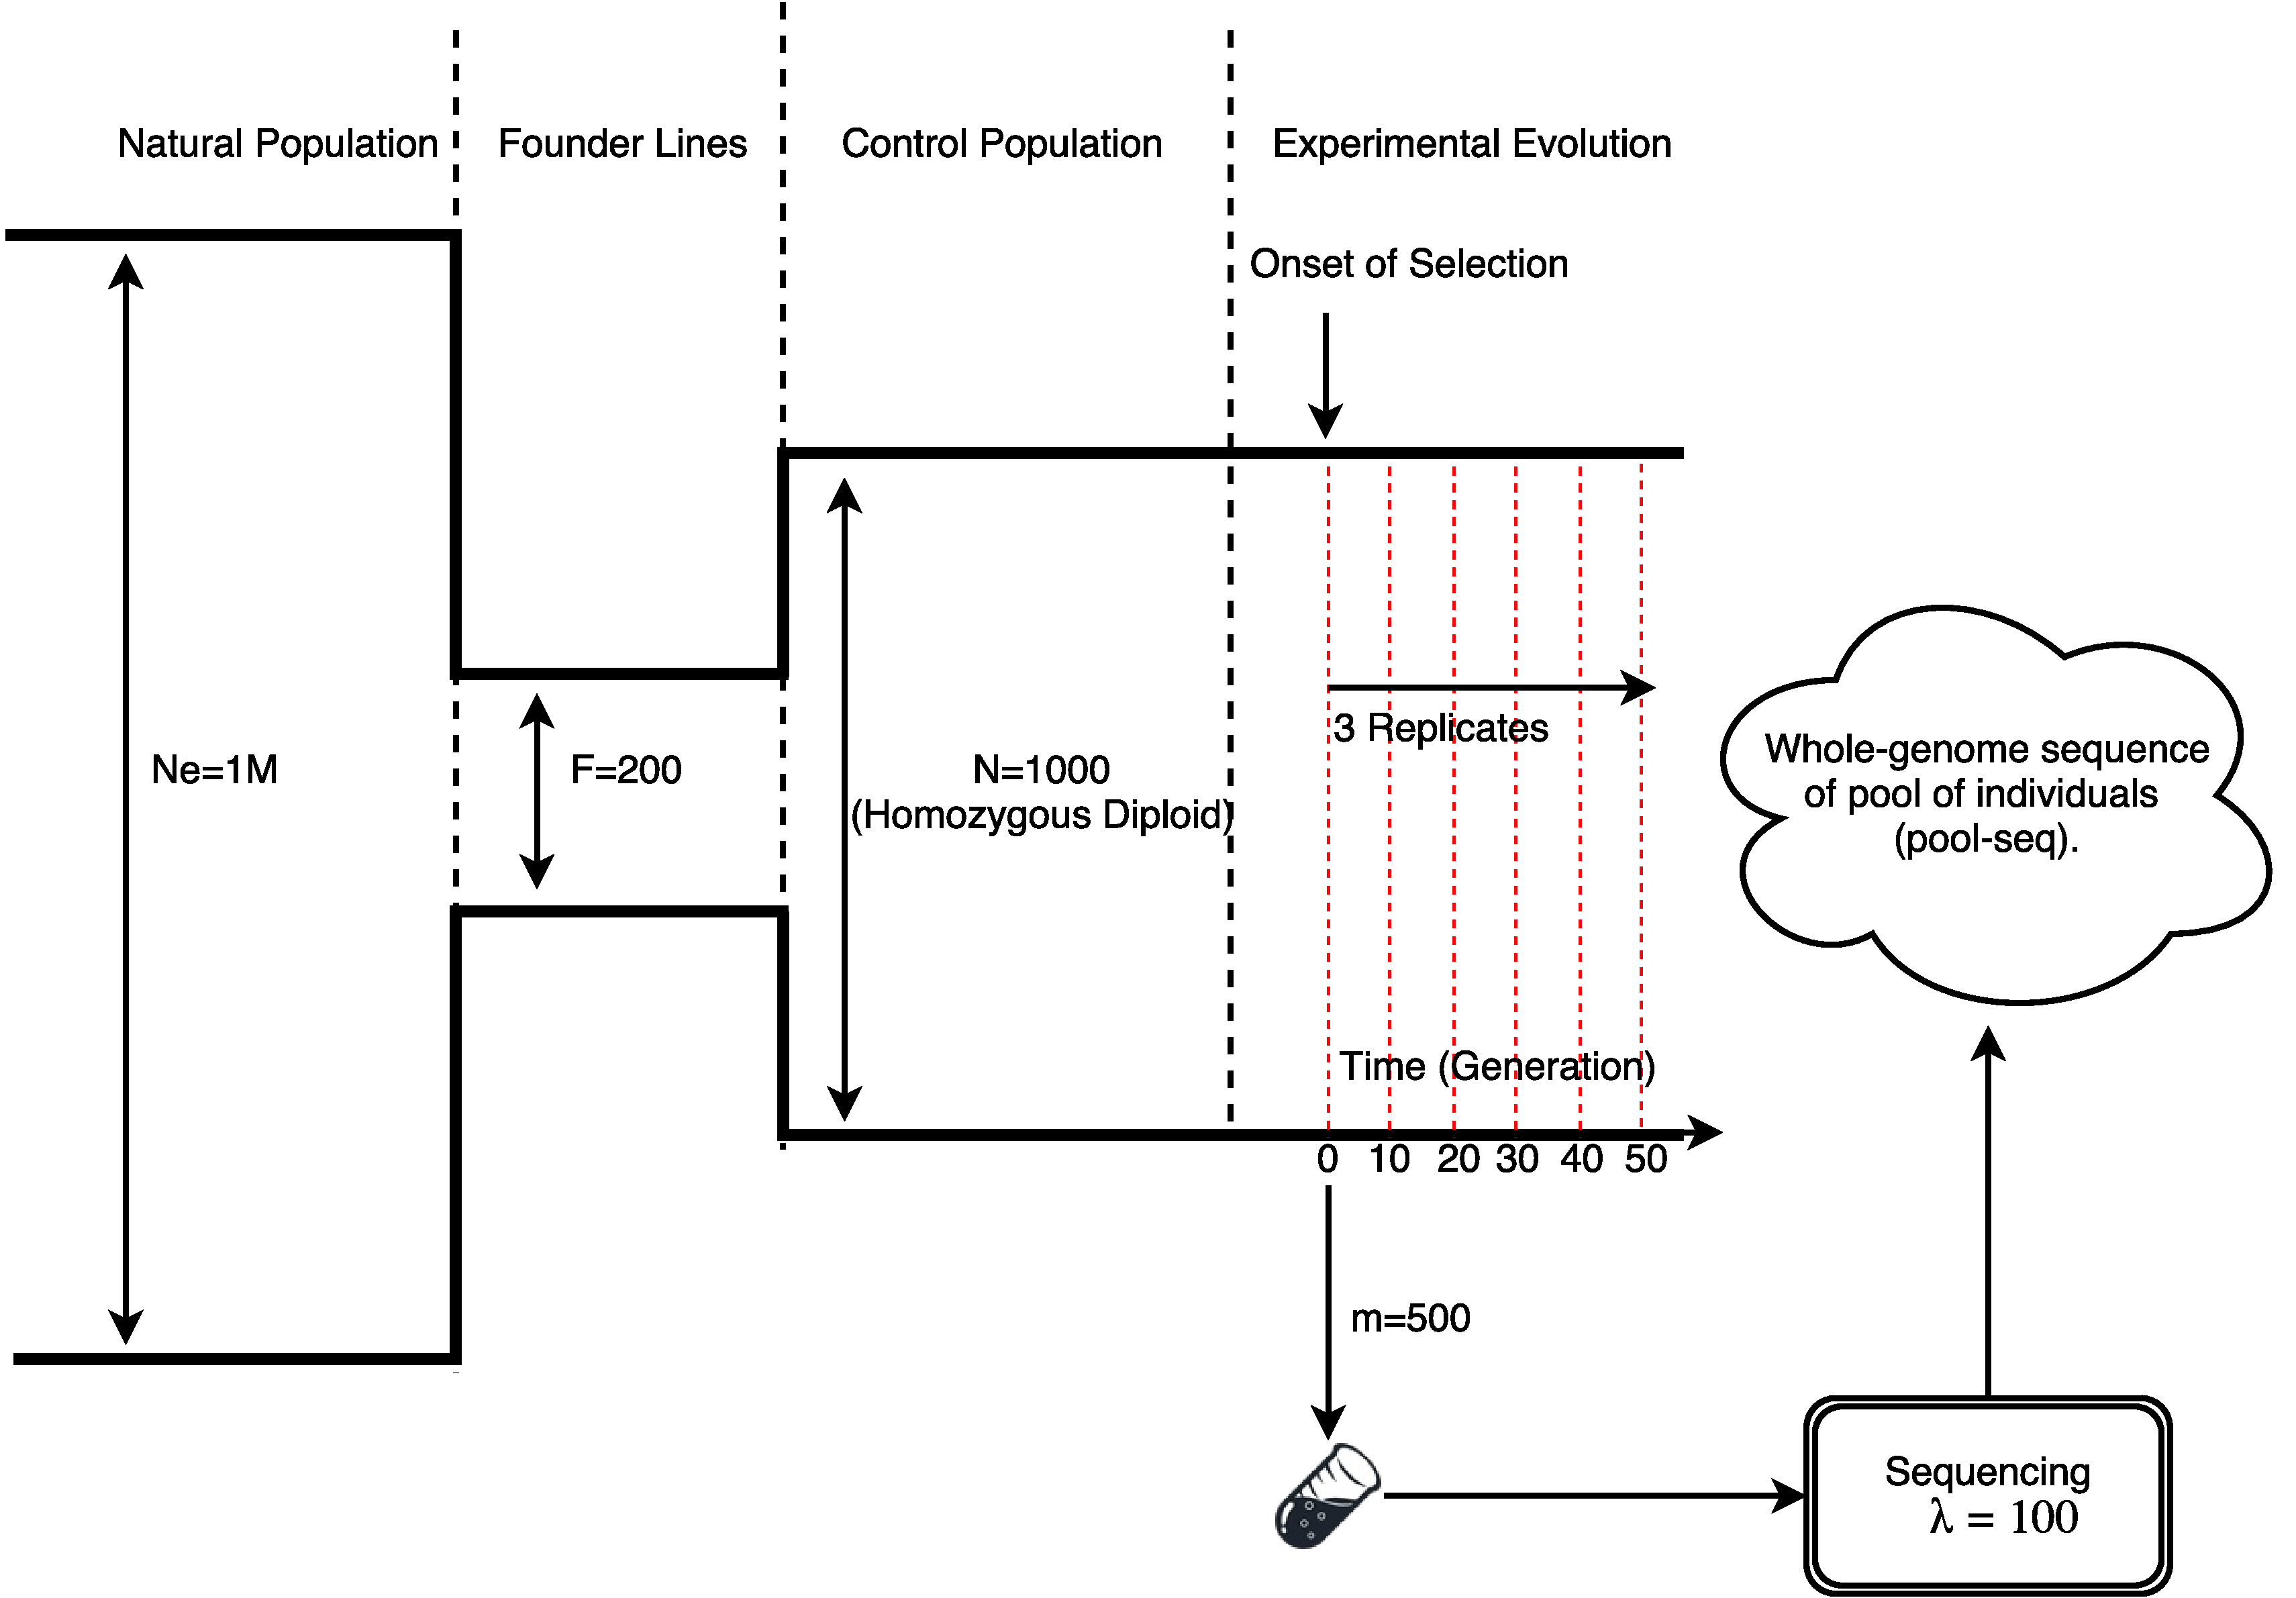
\includegraphics[trim=0.1in 0 .08in 0.02in , 
	clip,width=\textwidth]{figures/ExperimentalEvolution.pdf}
	\caption{ {\bf Two settings for collecting genomic time series
            data.}  Different settings in which dynamic data is
          collected are depicted with typical parameters for \emph{D.
            melanogaster}. In both settings, 6 samples (vertical red
          dashed lines) are taken every 10 generation.  When sampling
          from naturally evolving populations (A), the time of onset
          of selection is unknown, and population size is larger. For
          (controlled) experimental evolution, founder lines are first
          sampled from a natural population to create a homogeneous
          population. Multiple replicates of this population are
          evolved and sampled over time. }
	\label{fig:ee}
\end{figure}


\begin{figure}[H]
	\centering
	\includegraphics[width=\textwidth]{figures/{markovDists}.pdf}
        \caption{{\bf Comparison of empirical distributions of allele
            frequencies (green) versus predictions from Brownian
            Motion (red), and Markov chain (blue).} Panels A-F:
          Experiments were conducted under neutral evolution with
          different starting frequencies $\nu_0\in\{0.005,0.1\}$ and
          sampling times $\tau \in \{1,10,100\}$ generations. The
          empirical distribution was computed by sampling 143,900
          sites with $\nu_0=0.005$ and 47,500 variants with
          $\nu_0=0.1$. Panels G,H,I: Comparisons of Empirical and
          Markov chain based allele frequency distributions under a
          selection regime with $s=0.1$. Initial frequency was chosen
          as $\nu_0=0.005$ and sampling performed after $\tau$
          generations for $\tau \in \{1,10,100\}$.}
	\label{fig:markov}
\end{figure}

\begin{figure}[H]
	\centering
	\includegraphics[trim=.2in 0 .2in 0, 
	clip,width=\textwidth]{figures/{CLRQ}.pdf}
	\caption{{\bf Average power of composite statistics as function of 
	percentile cutoffs.} Detection power is averaged for 
	$s\in\{0.025,0.05,0.075,0.1\}$ using \comale statistic computed using 
	modified likelihood ration $\Hc(H)$ and standard likelihood ratio 
	$\Hc(|H|)$. For each setting the best performance is gained at  $\pi^*$ 
	which is different for different settings. As expected, $\pi^*$ takes 
	larger value (due to lower LD of the variation with favored allele). In 
	addition, for low coverage experiment better performance is achieved when 
	more candidate SNPs are take into computation of the composite statistic, 
	i.e., $\pi^*$ is lower. }
	\label{fig:clrq}
\end{figure}

\begin{figure}[H]
	\centering
	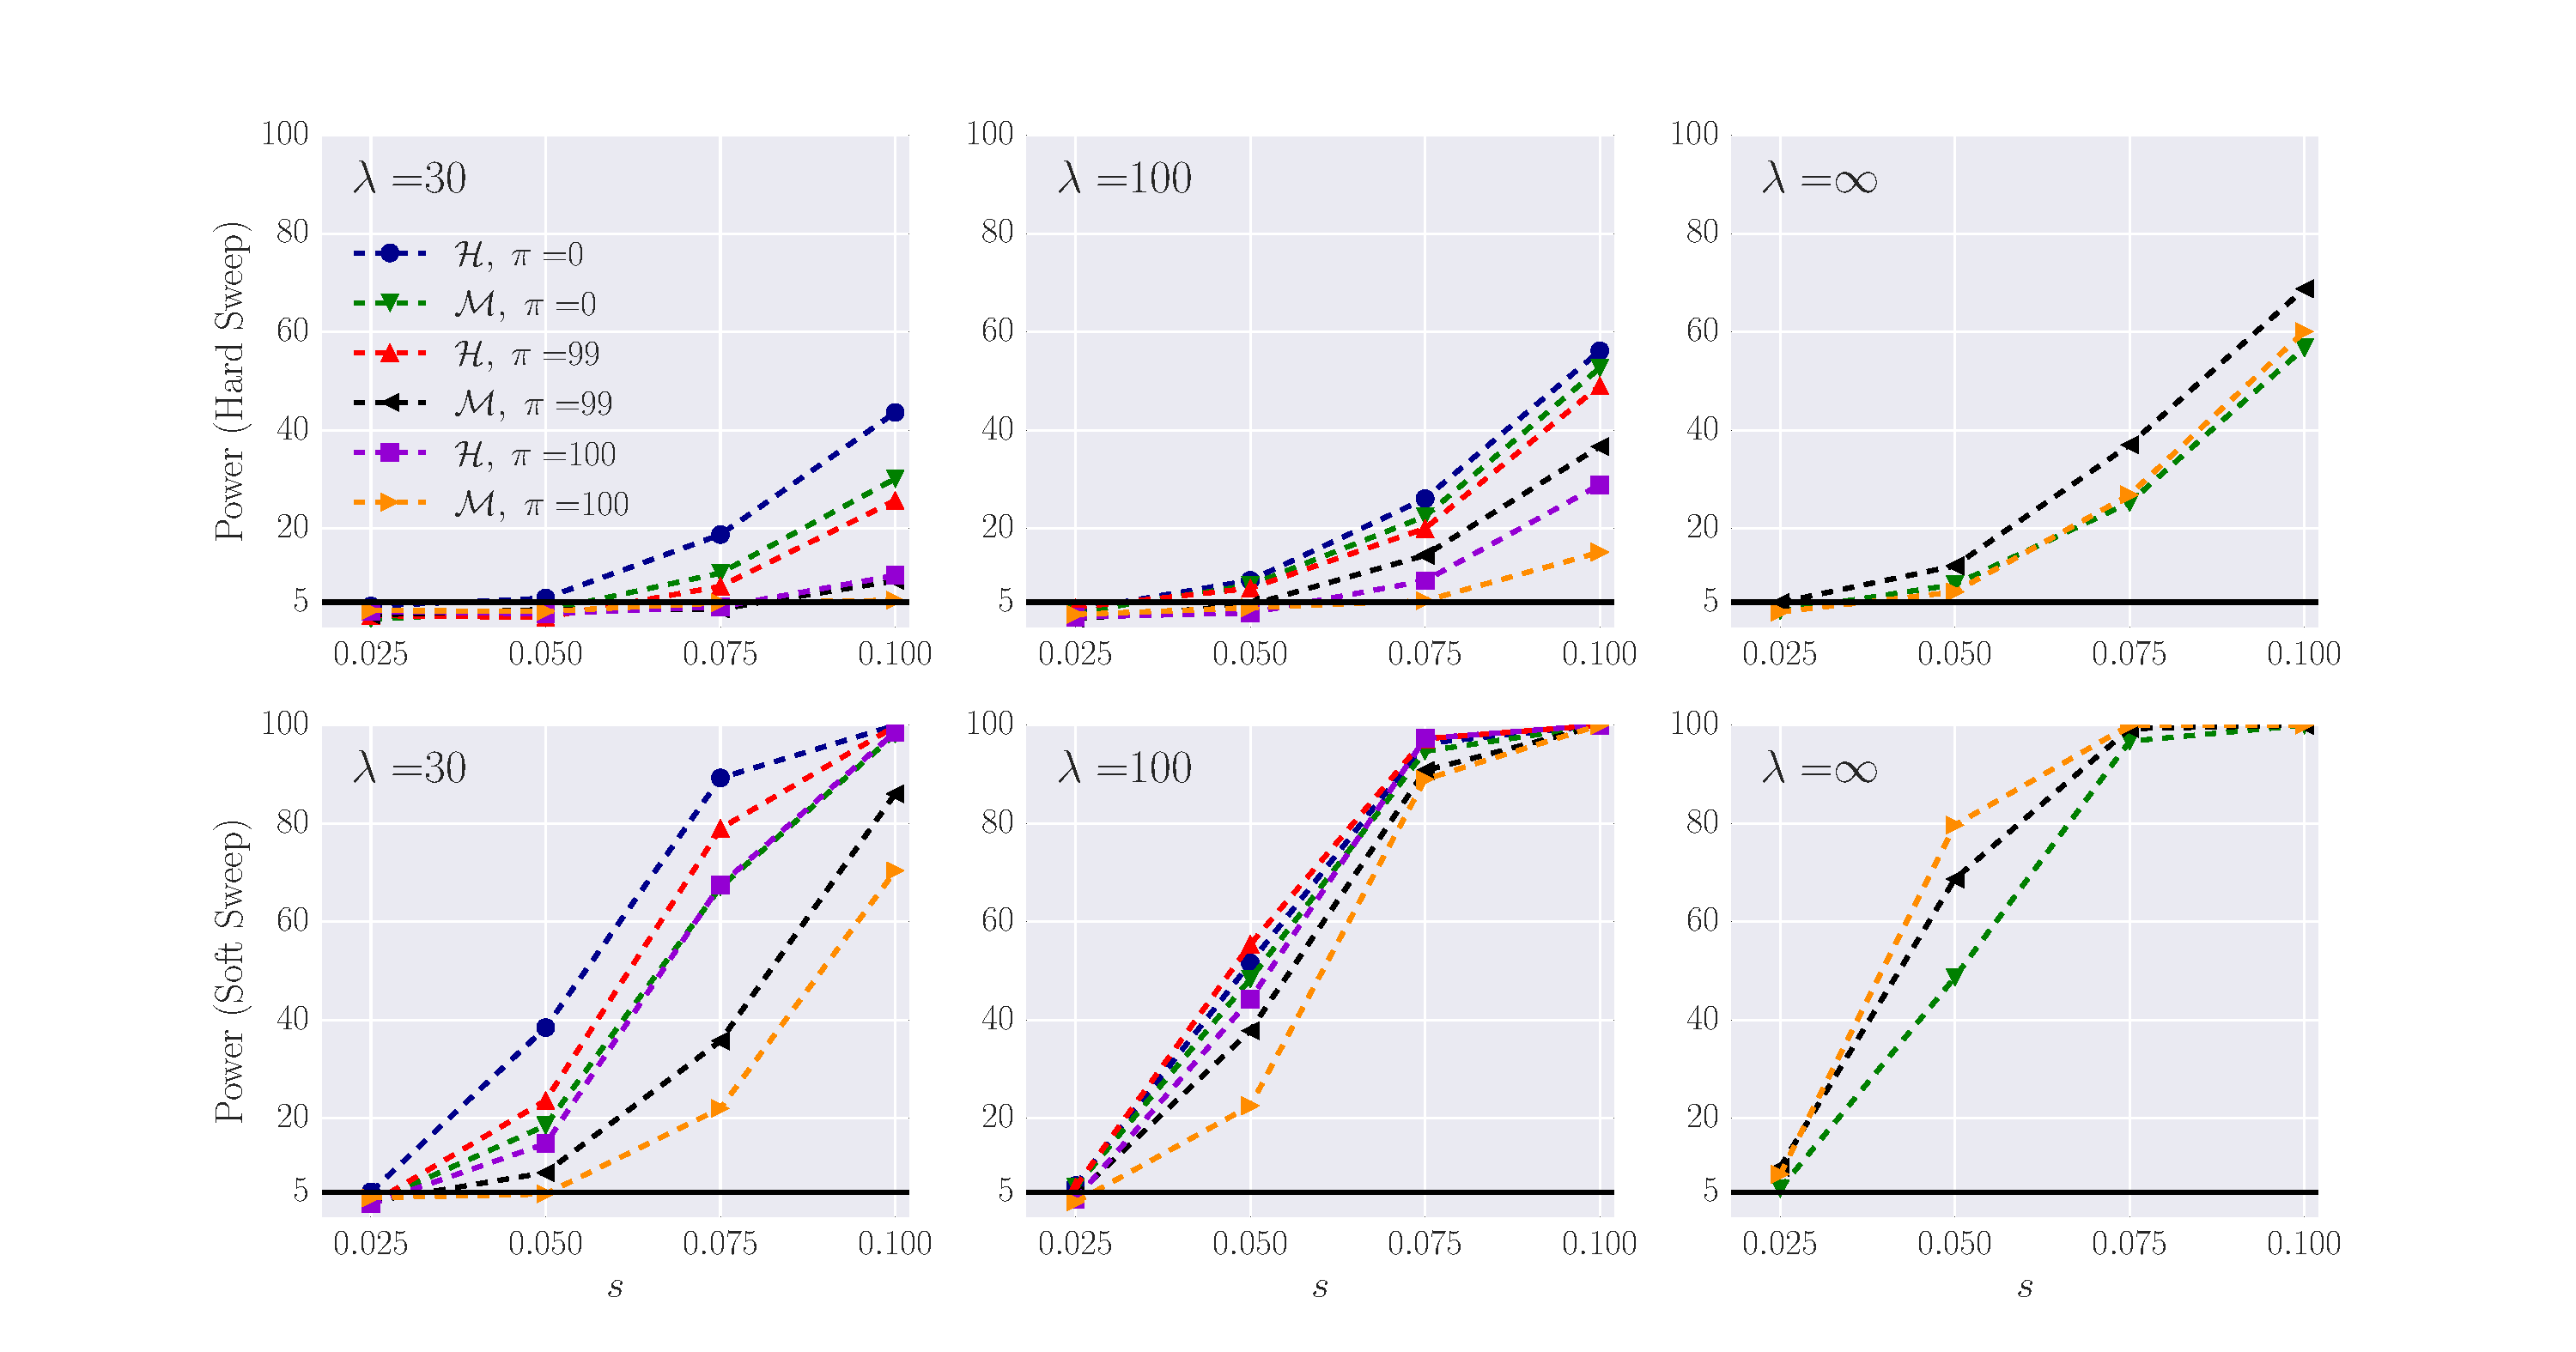
\includegraphics[width=\textwidth]{figures/powerCLR.pdf}
	\caption{{\bf Detection power of \comale-M and \comale-H with
            different composite statistics.}  Detection power for
          \comale-M ($\Mc$) and \comale-H ($\Hc$) under hard (top) and
          soft sweep (bottom) scenarios, for different settings of
          mean coverage $\lambda$ and selection strength $s$.  The
          $y$-axis measures power -- sensitivity with false positive
          rate FPR $\le 0.05$ -- for $1,000$ simulations of $50$Kbp
          regions.  } \label{fig:powerCLR}
\end{figure}

\begin{figure}[H]
	\centering
	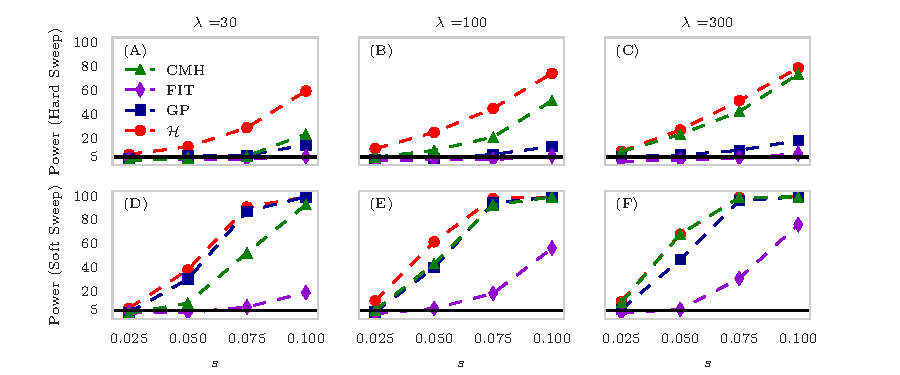
\includegraphics[width=\textwidth]{figures/power.pdf}
	\caption{ {\bf Power calculations for detection of selection.}
          Detection power for \comale ($\Hc$), Frequency Increment
          Test (FIT), Gaussian Process, and CMH under hard (top) and
          soft sweep (bottom) scenarios. $\lambda$, $s$ denote the
          mean coverage and selection coefficient, respectively. The
          $y$-axis measures power -- sensitivity with false positive
          rate FPR $\le 0.05$ -- for $1,000$ simulations of $50$Kbp
          regions. } \label{fig:power}
\end{figure}

\clearpage
\newpage
\begin{figure}[H]
	\centering
	\includegraphics[width=0.75\textwidth]{figures/{runTime.pdf}}
	\caption{{\bf Running time}. Box plot of running times
          (CPU-secs.) of \comale, HMM, GP with single, 3, 5, 7, and 10
          loci over 1000 simulations conducted on a workstation with
          4th Generation Intel Core i7 processor. The average running
          time for each method is shown on the x-axis.}
	\label{fig:runTime}
\end{figure}
\clearpage
\newpage

\begin{figure}[H]
	\centering
	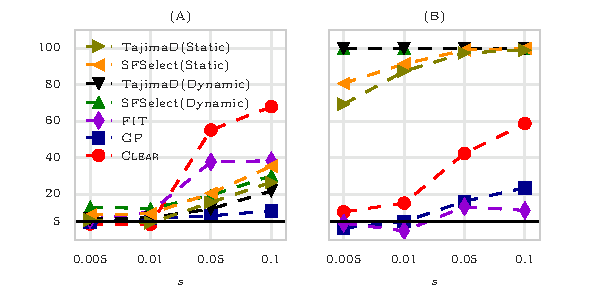
\includegraphics[width=0.7\textwidth]{figures/naturalee.pdf}
	\caption{{\bf Power of SFS based statistics.} Power of
          detecting selection for Frequency Increment Test (FIT),
          Gaussian Process (GP), \comale-H ($\Hc$) on hard-sweep
          natural experimental evolution with $N_e=10^4$ and depth
          $\lambda=\infty$. The measurements are conducted for a range
          of selection coefficients, $s$. Each point represents the
          mean of 200 simulations. For each simulation, sampling
          starts at a randomly chosen time, and subsequently 5
          replicate samples are acquired every $10$ generations.  (A)
          Start of sampling is chosen randomly throughout the sweep
          $\tau_1 \sim U\left[1,t_{\nu=1}(s,N_e)\right]$, where
          $t_{\nu=x}(s,N_e)$ denotes is the expected time to reach
          carrier frequency $x$ in a hard sweep and $U[a,b]$ is
          discrete uniform distribution. (B) The start of sampling is
          chosen near fixation of the favored allele, i.e. $\tau_1
          \sim
          U\left[t_{\nu=0.9}(s,N_e),t_{\nu=1}(s,N_e)\right]$.} 
          \label{fig:powerSFS}
\end{figure}

\clearpage
\newpage
\begin{figure}[H]
	\centering
	\includegraphics[trim=.2in 0 .2in 0, 
	clip,width=\textwidth]{figures/{rank100.0}.pdf}
	\caption{{\bf Ranking performance for 100X coverage.} Cumulative 
	Distribution Function (CDF) of the
          distribution of the rank of the adaptive allele in 500
          simulations for \comale-H, Gaussian Process (GP),
          CMH, and Frequency Increment Test (FIT), for different
          values of selection coefficient $s$ and initial carrier
          frequency. Area Under Curve (AUC) is computed as a
          quantitative measure ranking performance of methods for each
          configuration.}
	\label{fig:rank}
\end{figure}



\clearpage
\newpage
\begin{figure}[H]
	\centering
\includegraphics[width=0.7\textwidth]{figures/{bias.100}.pdf}
\caption{{\bf Distribution of bias for 100X coverage.} The
  distribution of bias ($s-\hat{s}$) in estimating selection
  coefficient over 500 simulations using Gaussian Process (GP) and
  \comale-H is shown for a range of choices for the selection
  coefficient $s$ and starting carrier frequency $\nu_0$, when
  coverage is 100.  The estimation performance of GP and HMM are very
  similar in soft sweep, while HMM provides lower variance in hard
  sweep(overall standard deviation is 0.036 for GO and is 0.028 for
  HMM).  }
	\label{fig:bias100}
\end{figure}

\clearpage
\newpage
\begin{figure}[H]
	\centering
	\includegraphics[width=\textwidth]{figures/{manhattan.min500snp}.pdf}
	\caption{{\bf \comale\ scan of the \data.}. Manhattan plot of the composite 
	$\Hc$
          statistic (A) and the number of SNPs (B) in 50Kbp
          sliding window with steps of 10Kbp, excluding windows close
          to centromere and telomere. The dashed line corresponds to
          the top $1$\%-ile cut-off and the candidate regions above the 
          threshold are show 
          in red dots. For comparison to past results,
          only Chromosomes 2, 3, and X are shown.}
	\label{fig:manhattancutoffed}
\end{figure}

\clearpage
\newpage

\clearpage
%
%%%%%%%%%%%%%%%%%%%%%%%%%%%%%%%%%%%%%%%%%%%%%
%%%%%%%%%%%%%%%%%%% Supplemental Material%%%%
%%%%%%%%%%%%%%%%%%%%%%%%%%%%%%%%%%%%%%%%%%%%%
\clearpage
%\newpage
%\setcounter{page}{1}
\setcounter{figure}{0}
\setcounter{table}{0}
\setcounter{equation}{0}
\renewcommand{\thefigure}{S\arabic{figure}}
\renewcommand{\thetable}{S\arabic{table}}
\renewcommand{\theequation}{S\arabic{equation}}

%\section*{Main text figure captions}
%\section*{Supporting information captions}
\section{Appendix}
\subsection{An approximate logistic function  for allele frequency dynamics} 
\label{app:af}
Assume that a site is evolving under selection constraints $s,h\in
\Rbb$, where $s$ and $h$ denote selection strength and overdominance,
respectively. Let $\nu_t$ denote the frequency of the site at time
$\tau_t\in {\cal T}$. Then, $\nusp$, the frequency at time $\tau_t+1$
can be estimated (See Eq.~\ref{eq:transition}) using:
\[\hat{\nu}_{t^+}
=\nu_t+\frac{s(h+(1-2h)\nu_t)\nu_t(1-\nu_t)}{1+s\nu_t(2h+(1-2h)\nu_t))}.
  \label{eq:transition}
\]
We can show that the dynamic of the favored allele can be modeled
via a logistic function, in the case of directional selection
($h=0.5$). Taking derivatives of Eq.~\ref{eq:transition}, we have
\beq \frac{\bfd \nu_t}{\bfd t} = \frac{s\nu_t(1-\nu_t)}{2+2s\nu_t}
\eeq To, solve the differential equation, note that for small $s$,
$2+2s\nu_t \approx 2$. Substituting,
\begin{equation}
\nu_t =\frac{1}{1+\frac{1-\nu_0}{\nu_0}e^{-st/2}} = \sigma(st/2+\eta(\nu_0)) 
\label{eq:inf-pop}
\end{equation}
where $\sigma(.)$ is the logistic function and $\eta(.)$ is logit function 
(inverse of the logistic function). 

\subsection{Dynamic of Tajima's $D$}\label{app:td}
In this part we derive dynamic of Tajima's $D$ statistic in \emph{hard
  sweep} as function of its value at the onset of selection, $D_0$,
selection strength and the frequency of the favored allele at the
onset of selection.  Let $D_0, \Pi_0, W_0$, be Tajima's $D$, Tajima's
estimate of $\theta$, and Watterson's estimate of $\theta$ at time
zero and $D_0=\Pi_0 - W_0$.  In order to compute, $D_t=\Pi_t - W_t$ we
compute $\Pi_t$ and $W_t$ separately as follows. Let $P$ be the $n
\times n$ matrix of pairwise heterozygosity of individuals, then
$\Pi={1}/{n^2}\sum P_{ij}$. So, if the population consist of $\nu
n$ identical carrier haplotype (due to lack of recombination), their
pairwise hamming distance is zero and should be subtracted from the
total $\Pi_t$: \beq \Pi_t&= (1-\nu_t^2)\Pi_0 \label{eq:tdt0} \eeq

To compute $W_t$, first remember that $W_t= \frac{m_t}{S_n}$ where
$m_t$ is the number of segregating sites at time $t$ and $S_n=
\sum_i^n 1/i \approx \log(n)$. Also we have \beq
\frac{W_t}{W_0}&=\frac{\frac{m_t}{S}}{\frac{m_0}{S}} \ \ \Rightarrow
W_t=\frac{m_t}{m_0}W0 \label{eq:tdt1} \eeq Because of hard sweep and
lack of recombination assumption, the population at time $t$ consist
of $(1-\nu_t)n$ non-carrier haplotypes and $\nu_tn$ identical carrier
haplotypes. While not strictly correct, we assume that the
$(1-\nu_t)n+1$ individuals are evolving neutrally. Using this
assumption, we have \beq \frac{m_t}{m_0}&=\frac{\log\left((1-\nu_t)n
    +1 \right)\theta}{\log(n)\theta} \approx
\frac{\log\left((1-\nu_t)n\right)}{\log(n)} =
\frac{\log(1-\nu_t)+\log(n)}{\log(n)} = 1+ \frac{
  \log(1-\nu_t)}{\log(n)}. \label{eq:tdt2} \eeq Finally, by putting
Eqs.~\ref{eq:tdt0},~\ref{eq:tdt1},~\ref{eq:tdt2} together, we can
explicitly write the dynmics of $D$ statistic as \beq D_t&=
(1-\nu_t^2)\Pi_0 - (1+ \frac{ \log(1-\nu_t)}{\log(n)} ) W_0 \\&=
D_0-\log(1-\nu_t) \frac{W_0}{\log(n)} -\nu_t^2 \Pi_0\\
&\approx D_0-\log(1-\sigma(st/2+\eta(\nu_0))) \frac{W_0}{\log(n)}
-\sigma(st/2+\eta(\nu_0))^2 \Pi_0.  \eeq where $\sigma$ and $\eta$ are
logistic and logit functions.


\subsection{Dynamics of Fay and Wu's H}\label{app:h}
%\bl
In any finite population size of $n$ with $m$ segregating sites,
allele frequencies take discrete values, i.e., $x_j \in
\{\frac{1}{n},\frac{2}{n},\ldots,\frac{n-1}{n}\}, \ \forall j
\in{1,\ldots,m}$. We have the following:
\begin{equation*} 
\|\bfx\|^2= \sum_{j=1}^{m} x_j^2
= \sum_{i=1}^{n-1}\left(\frac{i}{n}\right)^2\xi_i= \frac{ (n-1)}{2n}H,
\end{equation*} 
where $\xi_i$ is the number of sites with frequency $i/n$ and $H$ is
the Fay \& Wu's estimate of $\theta$ and $\bfx \in (0,1)^m$ is the
vector of allele frequency of a region with $m$ segregating
sites. Recently, Ronen \emph{et al.}~\cite{ronen2015predicting}
devised the $1\dHAF$ statistic for identifying selection on static
data, and showed that the expected value of $1\dHAF$ statistic is
given by:
\begin{equation} 
\Ebb[1\dHAF(t)]= n\| \bfx_t\|^2\approx ng(\nu_t)
\end{equation} 
where
\beq
g(\nu_t)= \theta \nu_t \left(\frac{\nu_t+1}{2} - \frac{1}{(1-\nu_t)n+1}\right) +
\theta (1-\nu_t)\left(\frac{n+1}{2n}-\frac{1}{(1-\nu_t)n+1}\right)
\label{eq:hafscorepooled}
\eeq
The dynamics of Fay \& Wu's estimate are given by
\beq
H_t=\frac{n-1}{2} g(\nu_t)
\eeq
\subsection{Greedy computation of time-series SFS-based  
statistics}\label{app:agg}
As discussed in Section~\ref{sec:extending-sfs}, modeling dynamic of
Tajima's $D$ (and Fay\&Wu's $H$) requires knowledge of initial carrier
frequency $\nu_0$ and the value of $D$ (and $H$) statistic at the
onset of selection, which are often unknown.  As these statistics are
monotonically decreasing (or increasing for SFSelect) under no
demographic changes, we chose to greedily aggregate statistics
throughout time. For example, for Tajima's $D$, we have \beq \Dc =
\sum_{t \in \Tc} D_t \eeq where the same procedure applies to
Fay\&Wu's $H$ and SFSelect.


\subsection{Linkage Disequilibrium}\label{app:ld}
Nonrandom associations, Linkage Disequilibrium (LD), between 
polymorphisms are established in the 
substitution process, broken by recombination events 
and reinforced by selection. 
Although LD can not be measured in pooled sequencing data (phased 
haplotype data is required), it is still worthwhile 
to examine the behavior of LD as a result of the interaction between 
recombination and natural selection. In this part we theoretically overview 
expected LD in short EEs.

Let $\rho_0$ be the LD at time zero between the favored allele and a 
segregating site $l$ base-pairs away, then under natural selection we have
\beq
\rho_t= \alpha_t\beta_t \rho_0=e^{-rtl} \left(\frac{K_t}{K_0}\right)  
\rho_0\label{eq:ldt}
\eeq
where $K_t=2\nu_t(1-\nu_t)$ is the heterozygousity at the selected site, $r$ is 
the recombination rate/bp/gen. The 
\emph{decay factor}, $\alpha_t=e^{-rtl}$,
and \emph{growth factor}, $\beta_t$ (see Eq. 30-31 in 
\cite{Stephan2006The}), are result of recombination and 
selection, respectively. Fig.~\ref{fig:ld3d} presents the expected theoretical 
value of LD when $\rho_0=0.5$ between favored allele (site at position 500K) 
and the rest of 
genome, and $\nu_0=0.1$. For neutral evolution (top), LD decays exponentially 
through space and time, while in natural selection (bottom), LD increases and 
then decreases. Interestingly, LD increases to its maximum value, 1, for the 
nearby region (the plateau in the Fig.~\ref{fig:ld3d} bottom) of the favored 
allele.

In principle, LD increases after the onset of selection, until $\log(\alpha_t) 
+\log(\beta_t) 
>0$, see Eq.~\ref{eq:ldt}. 
Specifically, log of decay term is linear and, using 
Eq.~\ref{eq:inf-pop}, we write growth 
factor in term of initial frequency $\nu_0$ and selection strength $s$. 
Fig.~\ref{fig:ldf} depicts interaction of decay and growth factors for weak and 
strong selection and soft and hard sweeps. In all the case, LD of the 
favored allele with a segregating site 50Kbp away, increases in the first 50 
generations, which give rise to increasing number of \emph{hitchhikers}. 

Increase of LD in a large (100Kbp) region is particularly advantageous to the 
task of identifying the region under selection, if the composite statistics is 
used. As a result, $\Hc$ statistic outperforms existing (single-loci) tools in 
identifying selection. In contrast, augmentation of LD, increases the 
number 
of candidates for 
the favored allele, which makes is difficult to localize the favored 
allele.

\clearpage
\newpage

\setcounter{figure}{0}
\setcounter{table}{0}
\setcounter{equation}{0}
\renewcommand{\figurename}{}
\renewcommand{\tablename}{}
\renewcommand{\thefigure}{S\arabic{figure} Fig}
\renewcommand{\thetable}{S\arabic{table} Table}
\renewcommand{\theequation}{S\arabic{equation}}

\clearpage
\newpage
\begin{figure}[H]
 \begin{algorithm}[H]
 	\SetAlgorithmName{Generative Process}
 	\DontPrintSemicolon
 	\SetAlgoNoLine
 	\KwIn{$N,n,R,\{\lambda_t\}_{t\in\Tc},\Tc= 
 		\{\tau_0,\ldots\tau_T\}$ }
 	\KwOut{Time-series pool-seq data for $R$ replicates of a single locus 
 		$\{\bfc\}_R$ and $\{\bfd\}_R$.}
 	\For{$r\leftarrow 1$ \KwTo $R$}
 	{
 		\For{$t\leftarrow \tau_0$ \KwTo $\tau_T$}
 		{
 			$2N\nu_t \sim \text{Binomial}({2N},{\nu_{t-1}})$\;
 			\If{$t\in \Tc$ }
 			{
 				$d^{(r)}_{t} \sim \poiss(\lambda_{\tau_i})$ \;
 				$2ny_t \sim \text{Binomial}({2n},{\nu_{t}})$\;  
 				$c^{(r)}_{t} \sim \text{Binomial}(d^{(r)}_{t},{y_{t}})$\; 
 			}
 		}
 	}
 	\caption{The Generative Process for Neutral Wright-Fisher 
 	Time-series Pool-seq Data.} 
 \end{algorithm}
 \caption{{\bf The Generative Process for Neutral Wright-Fisher 
 		Time-series Pool-seq Data.}}
  	\label{proc:arya}
\end{figure}	
\begin{figure}[H]
	\centering
	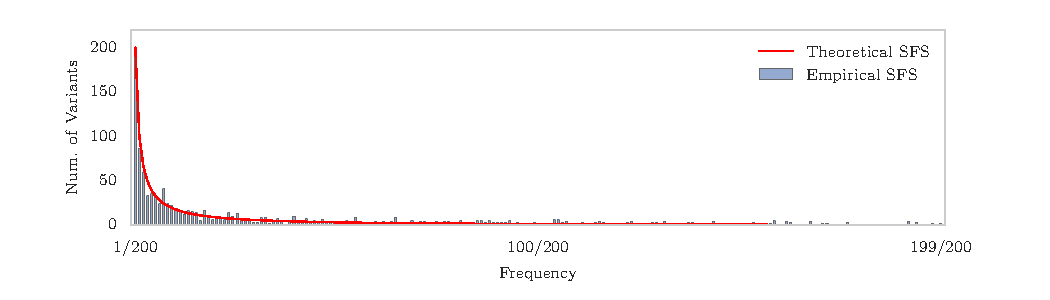
\includegraphics[trim=.01in 0.1in .01in 
	0.1in,clip,width=\textwidth]{sfs.pdf}
	\caption{{\bf Site Frequency Spectrum.}\\ Theoretical and
          Empirical SFS in a 50Kbp region for a neutral population of 200
          individuals when $N_e=10^6$ and $\mu=10^{-9}$. The $x$-axis 
          corresponds to site frequency, and
          the $y$-axis to the number of variants with a specific
          frequency. 
          In a neural population, majority of the variations stand in low 
          frequency.} \label{fig:sfs}
\end{figure}

\ignore{
\begin{figure}[H]
	\centering
	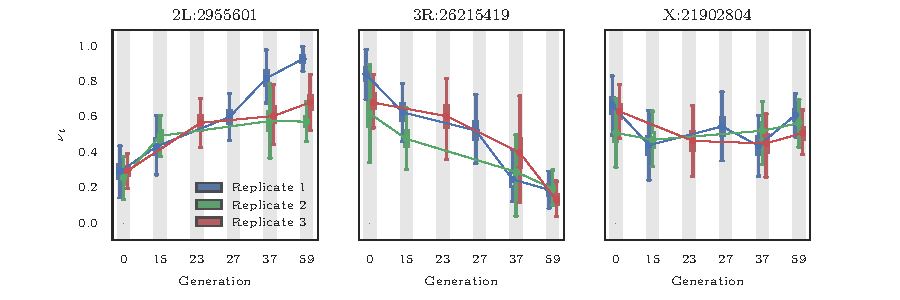
\includegraphics[width=\textwidth]{trajectoryReal.pdf}
	\caption{{\bf Trajectory of pool-sequenced variants.}\\
		Trajectory of three different variants that are increasing
		in frequency over time. Note that for read count data, the
		true allele frequency is not known. Here we draw the
		posterior distribution of the allele frequency at each time
		point using box plot. The median of each distribution is
		denoted by dots. The variance of each box is seen to be
		inversely related to the depth of the measurement. For instance, 
		generation 59 is sequenced with higher coverage than generation 37. 
		As a result, variance of observations in generation 59 is 
		considerably 
		smaller.}
	\label{fig:trajectoryReal}
\end{figure}
\begin{figure}[H]
	\centering
	\includegraphics[trim=.0in 0 .0in 0, 
	clip,width=0.5\textwidth]{{statePosterior}.pdf}
	\caption{{\bf Posterior distribution of allele frequency.}\\
		Distribution of hidden allele frequency for different values
		of depth $d=\{5,50,500\}$. In all cases, the true frequency
		is $0.2$. The estimated frequency values are binomially distributed, 
		with different variances,
		around the true value in all cases with.}
	\label{fig:stateConditional}
\end{figure}}
\begin{figure}[H]
	\centering
	\begin{tabular}{c}
		\includegraphics[trim=.2in 0 .0in 0, 
		clip,width=0.8\textwidth]{{depthHetero}.pdf}
	\end{tabular}
	\caption{{\bf Coverage heterogeneity in time series data.}\\ Each panel
		shows the read depth for 3
		replicates of the \datadm\ data (see section~\ref{sec:dmel}). 
		Heterogeneity in depth of coverage is 
		seen
		between replicates, and also at different time points, in
		all 4 variants. None of these sites pass the the hard filtering with 
		minimum depth of 30. }
	\label{fig:depthHetero}
\end{figure}


\begin{figure}[H]
	\centering
	\includegraphics[width=0.6\textwidth]{{slikes}.pdf}
	\caption{{\bf Likelihoods of the parameter $s$.}\\ 
		Likelihood of the parameter $s$ in \dmel data for a variant with 
		$\hs=0.2$ (A) and $\hs=0$ (B). 
		}
	\label{fig:slikes}
\end{figure}


\begin{figure}[H]
	\centering
		\includegraphics[width=0.6\textwidth]{{bias.30}.pdf}
	\caption{{\bf Distribution of bias for 30$\times$ coverage.}\\ The
		distribution of bias ($s-\hat{s}$) in estimating selection
		coefficient over 1000 simulations using Gaussian Process (GP) and
		\comale\ ($H$) is shown for a range of choices for the selection
		coefficient $s$ and starting carrier frequency $\nu_0$, when
		coverage $\lambda=30$ (Panels A,B). GP and \comale\ have similar
		variance in estimates of $s$ for soft sweep, while \comale\ provides
		lower variance in hard sweep. Also see \ref{tab:biasdist}. Panels 
		C,D
		show the variance in the estimation of $h$.}
	\label{fig:bias30}
\end{figure}


\begin{figure}[H]
	\centering
	\includegraphics[width=0.6\textwidth]{{bias.300}.pdf}
	\caption{{\bf Distribution of bias for 300$\times$ coverage.}\\ The
		distribution of bias ($s-\hat{s}$) in estimating selection
		coefficient over 1000 simulations using Gaussian Process (GP) and
		\comale\ ($H$) is shown for a range of choices for the selection
		coefficient $s$ and starting carrier frequency $\nu_0$, when
		coverage $\lambda=\infty$ (Panels A,B). GP and \comale\ have similar
		variance in estimates of $s$ for soft sweep, while \comale\ provides
		lower variance in hard sweep. Also see \ref{tab:biasdist}. Panels 
		C,D
		show the variance in the estimation of $h$.
	}
	\label{fig:biasinf}
\end{figure}
\ignore{
\begin{figure}[H]
	\centering
	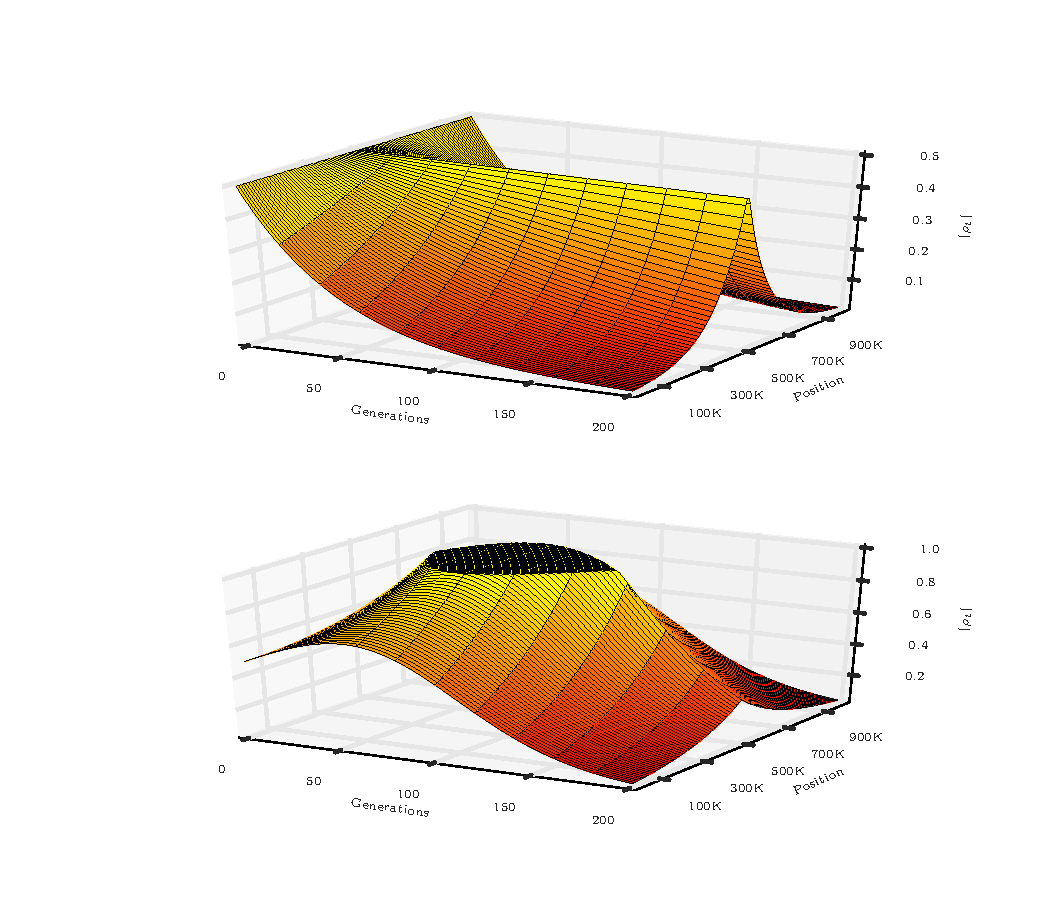
\includegraphics[width=\textwidth]{LDDecay3d}
	\caption{ {\bf Expected dynamic of LD under selection and neutral 
	evolution.}\\ Dynamic of LD ($\rho_t$) of a 1Mbp genome to the favored 
	allele 
	(at position 500K) is drawn as function of position and time for neutral 
	(top) and selection(bottom) regimes.
	For sake of illustration, we assumed that at generations 0, LD of all 
	variants with the favored allele is 0.5, initial frequency of the favored 
	allele is 0.1, recombination rate is $r=2\times10^{-8}$ (top). The 
	selection strength is 0 and 0.05 for neutral and selection regimes, 
	respectively. As expected LD decay exponentially  through space and time. 
	However, selection causes LD to increase then decrease.}	
		\label{fig:ld3d}
\end{figure}
}

\begin{figure}[H]
	\centering
		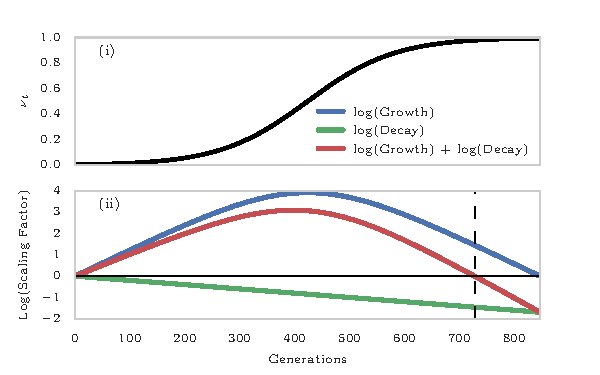
\includegraphics[width=0.8\textwidth]{decayFactors0}	
	\caption{{\bf Interaction between growth and decay factors of LD in 
	hard 
	sweep with	weak selection.}\\
		Expected dynamics of LD between favored allele and a variant 
		50Kbp 
		away, under weak selection ($s=0.025$) and hard 
		sweep 
		($\nu_0=0.005$). In addition to 
		recombination, initial frequency of the favored allele and selection 
		strength determine the dynamics of LD.
		The horizontal black line denotes the equilibrium between decay 
		and scaling factor.
		 The vertical dashed line represent the time in which decay and 
		 growth factors stay at equilibrium, after onset of selection.} 
		 \label{fig:ldf0}
\end{figure}

\begin{figure}[H]
	\centering
	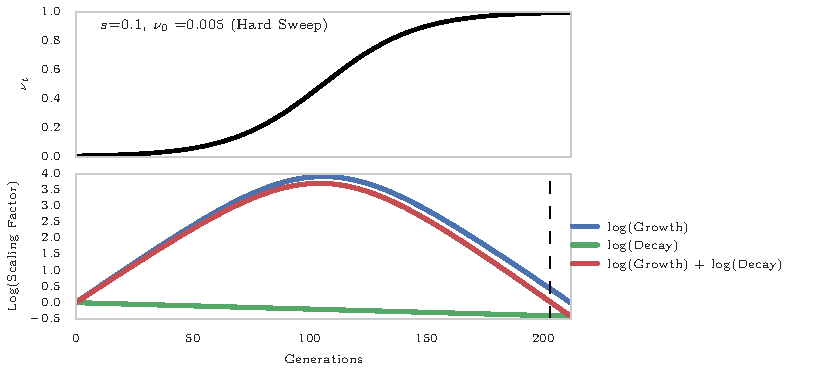
\includegraphics[width=0.8\textwidth]{decayFactors1}	
\caption{{\bf Interaction between growth and decay factors of LD in 
hard 
		sweep with	strong selection.}\\
	Expected dynamics of LD between favored allele and a variant 50Kbp 
	away, under strong selection ($s=0.1$) and hard sweep 
	($\nu_0=0.005$). In addition to 
	recombination, initial frequency of the favored allele and 
	selection 
	strength determine the dynamics of LD. The vertical dashed line 
	denotes 
	the time in which LD start to decrease. 		The horizontal 
	black line denotes the equilibrium between decay 
	and scaling factor.
	The vertical dashed line represent the time in which decay and 
	growth factors stay at equilibrium, after onset of selection.} 
	\label{fig:ldf1}
\end{figure}
\begin{figure}[H]
	\centering
	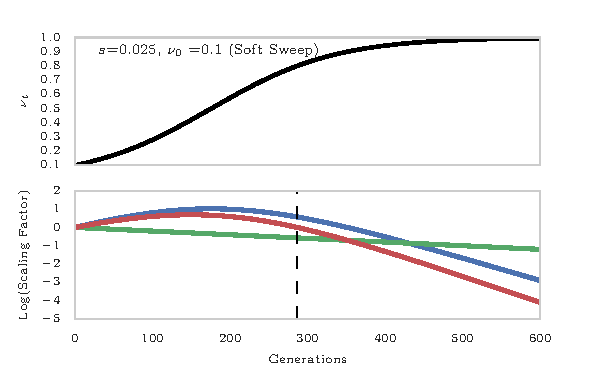
\includegraphics[width=0.8\textwidth]{decayFactors2}	
\caption{{\bf Interaction between growth and decay factors of LD in 
soft 
		sweep with	weak selection.}\\
	Expected dynamics of LD between favored allele and a variant 50Kbp 
	away, under weak selection ($s=0.025$) and soft sweep 
	($\nu_0=0.1$).  In addition to 
	recombination, initial frequency of the favored allele and 
	selection 
	strength determine the dynamics of LD. The vertical dashed line 
	denotes 
	the time in which LD start to decrease. 		The horizontal 
	black line denotes the equilibrium between decay 
	and scaling factor.
	The vertical dashed line represent the time in which decay and 
	growth factors stay at equilibrium, after onset of selection.} 
	\label{fig:ldf2}
\end{figure}
\begin{figure}[H]
	\centering
	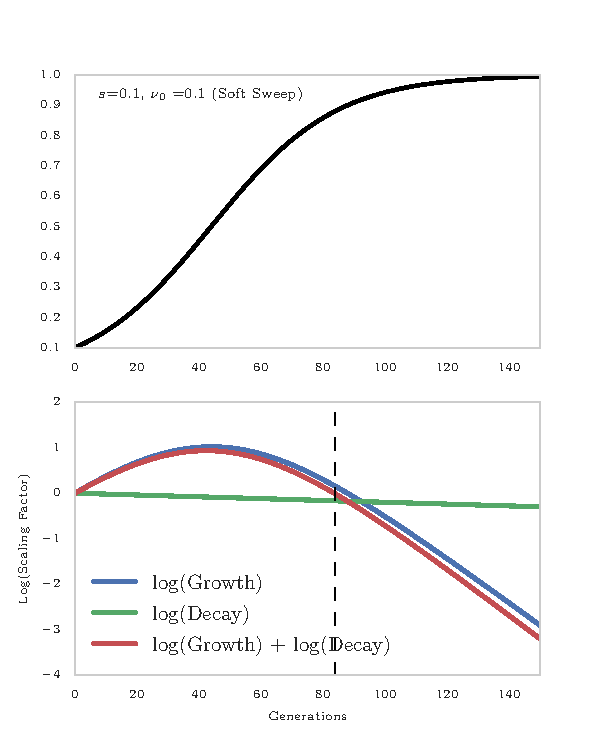
\includegraphics[width=0.8\textwidth]{decayFactors3}	
\caption{{\bf Interaction between growth and decay factors of LD in 
soft 
		sweep with	strong selection.}\\
	Expected dynamics of LD between favored allele and a variant 50Kbp 
	away, under strong selection ($s=0.1$) and soft sweep 
	($\nu_0=0.1$).  In addition to 
	recombination, initial frequency of the favored allele and 
	selection 
	strength determine the dynamics of LD. The vertical dashed line 
	denotes 
	the time in which LD start to decrease. 		The horizontal 
	black line denotes the equilibrium between decay 
	and scaling factor.
	The vertical dashed line represent the time in which decay and 
	growth factors stay at equilibrium, after onset of selection.} 
	\label{fig:ldf3}
\end{figure}


\begin{figure}[H]
	\centering
	\includegraphics[trim=.2in 0 .2in 0, 
	clip,width=\textwidth]{{rank30.0}.pdf}
	\caption{{\bf Ranking performance for 30$\times$ coverage.}\\
           Cumulative Distribution Function (CDF) of the distribution
           of the rank of the favored allele in 1000 simulations for
           \comale\ ($H$ score), Gaussian Process (GP), and Cochran 
           Mantel 
           Haenszel  
           (CMH), for different values of selection
           coefficient $s$ and initial carrier frequency.}
	\label{fig:rank300}
\end{figure}
\begin{figure}[H]
	\centering
	\includegraphics[trim=.2in 0 .2in 0, 
	clip,width=\textwidth]{{rank300.0}.pdf}
	\caption{{\bf Ranking performance for 300$\times$ coverage.}\\
           Cumulative Distribution Function (CDF) of the distribution
           of the rank of the favored allele in 1000 simulations for
           \comale\ ($H$ score), Gaussian Process (GP), and Cochran 
           Mantel 
           Haenszel  
           (CMH), for different values of selection
           coefficient $s$ and initial carrier frequency.}
	\label{fig:rankinf}
\end{figure}


\begin{figure}[H]
	\centering
	\includegraphics[width=0.7\textwidth]{{winSize}.pdf}
	\caption{{\bf Window size for $Ns$.}  The selected window size (XXX)
          as a function of $Ns$ for \dmel study with
          $\tau=59,N=250,r=2\times10^{-8}$.  }
	\label{fig:winSize}
\end{figure}








\begin{figure}[H]
	\centering
	\includegraphics[trim=.0in 0in .2in 0in, 	
	clip,width=0.9\textwidth]{{null-alt-dmel}.pdf}
	\caption{{\bf Distribution of $p$-values.}
		Distribution of $p$-values of \comale\ in null simulations and 
		experimental data when $N=250$. Panel (A),(C) shows the effect of under 
		estimations ($\hN=100$) and over-estimation ($\hN=500$) of population 
		size in computing $p$-values, and panel (B) shows the distribution of 
		$p-$values when unbiased estimate is used to create simulations.
		.}
	\label{fig:null-alt}
\end{figure}


\begin{figure}[H]
	\centering
	\begin{tabular}{cc}
		(A)&(B)\\
		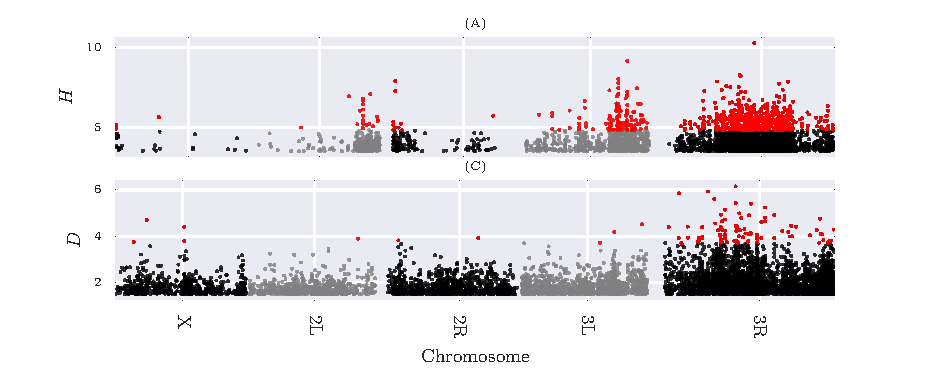
\includegraphics[trim=0.4in 0.in 0.6in 
		1.17in,clip,width=0.6\textwidth]{man-dmel-snp.pdf}&	
		\includegraphics[trim=0.1in 0.in 0in 
		1.5in,clip,width=0.35\textwidth]{{topVariants.dmel}.pdf}
	\end{tabular}
	\caption{{\bf Single locus analysis of the \datadm.}\\
	Manhattan plot of scan for
		testing dominant selection (A).  Significant variants
		with FDR $\le 0.01$ are denoted in red, and their
		trajectories are depicted in panel (B).}
	\label{fig:man-dmel-snp}
\end{figure}

\begin{figure}[H]
\begin{tabular}{cc}
	\includegraphics[width=0.5\textwidth]{{SFS.Y.G0}.pdf}&
	\includegraphics[width=0.5\textwidth]{{SFS.Y.G180}.pdf}\\
	\includegraphics[width=0.5\textwidth]{{SFS.Y.G360}.pdf}&
	\includegraphics[width=0.5\textwidth]{{SFS.Y.G540}.pdf}
\end{tabular}
\caption{{\bf Site frequency spectrum of the Yeast dataset.}
	Whole-genome site frequency spectrum of the Yeast dataset at generations 0 
	(A), 180 (B), 
	360 (C) and 540 (D). Some replicates, e.g. replicate 2, undergoing severe 
	demographic events.
	}
\label{fig:yeast-sfs}
\end{figure}

\begin{figure}[H]
	\centering
		\includegraphics[width=0.7\textwidth]{{PCA}.pdf}
	\caption{{\bf Population similarity.}
		Principle component analysis of the 12 replicates throughout the 
		experiment, showing that some populations exhibiting distinct frequency 
		spectra.
		}
	\label{fig:yeast-pca}
\end{figure}








\begin{table}[H]
	\centering
		\caption{\bf Average of power for detecting selection.}
	\begin{tabular}{ccc}
		Hard Sweep & &Soft Sweep\\ \\  
		\centering \begin{tabular}{c|c|c}
$\lambda$	&Method	&Avg Power\\\hline
100	&$\mathcal{H}$	&30\\
$\infty$	&$\mathcal{H}$	&29\\
30	&$\mathcal{H}$	&23\\
100	&CMH	&19\\
30	&CMH	&10\\
$\infty$	&GP	&7\\
100	&GP	&7\\
30	&GP	&7\\
$\infty$	&FIT	&5\\
100	&FIT	&4\\
30	&FIT	&3\\
\end{tabular}

		&&\centering \begin{tabular}{c|c|c}
$\lambda$	&Method	&Avg Power\\\hline
100	&$\mathcal{H}$	&64\\
$\infty$	&$\mathcal{H}$	&63\\
$\infty$	&GP	&60\\
100	&GP	&60\\
100	&CMH	&59\\
30	&$\mathcal{H}$	&58\\
30	&GP	&56\\
30	&CMH	&44\\
$\infty$	&FIT	&36\\
100	&FIT	&21\\
30	&FIT	&7\\
\end{tabular}

	\end{tabular}
	\caption*{		Average power is computed  for 8000 simulations 
	with 
		$s\in\{0.025,0.05,0.075,0.1\}$. Frequency Increment 
		Test (FIT), Gaussian Process (GP), \comale\ ($\Hc$ statistic) and 
		Cochran Mantel Haenszel (CMH) are compared for different initial 
		carrier frequency $\nu_0$. For all sequencing coverages, \comale\ 
		outperform other methods. When coverage is not high 
		($\lambda\in\{30,100\}$) and initial frequency is low (hard sweep), 
		\comale\ significantly perform better than others.}
	\label{tab:power}
\end{table}


\begin{table}[H]
	\centering
		\caption{\bf Average running time per variant in seconds for 
		different 
			methods.}
	\begin{tabular}{c}
		\centering \begin{tabular}{c|c}
Method	&Avg. Time per Variant\\\hline
CMH	&0.001\\
$\mathcal{M}$	&0.006\\
FIT	&0.006\\
$\mathcal{H}$	&0.042\\
GP(1)	&2.551\\
GP(3)	&19.177\\
GP(5)	&50.291\\
GP(7)	&95.602\\
GP(10)	&202.017\\
\end{tabular}

	\end{tabular}
\label{tab:times}
\end{table}

\begin{table}[h]
	\centering
	\caption{\bf Mean and standard deviation of the distribution of 
	bias 
		($s-\hat{s}$) of 8000 simulations with coverage 
		$\lambda=100\times$ and 
		$s\in\{0.025,0.05,0.075,0.1\}$.}
	\begin{tabular}{c}
		\centering \begin{tabular}{c|c|c|c|c}
index	&GP	&GP	&HMM	&HMM\\\hline
	&0.005	&0.1	&0.005	&0.1\\
	&	&	&	&\\
count	&2000.0	&2000.0	&2000.0	&2000.0\\
mean	&0.041	&0.0	&-0.003	&0.0\\
std	&0.036	&0.013	&0.028	&0.013\\
min	&-0.056	&-0.042	&-0.095	&-0.046\\
25\%	&0.018	&-0.009	&-0.02	&-0.009\\
50\%	&0.039	&-0.0	&-0.005	&-0.0\\
75\%	&0.062	&0.009	&0.015	&0.009\\
max	&0.25	&0.05	&0.1	&0.056\\
\end{tabular}

	\end{tabular}
	\label{tab:biasdist}
\end{table}

\clearpage
\newpage
\begin{table}[H]
	\centering
	\caption{\bf GO enrichment analysis of \datadm using 
		\texttt{Gowinda}.}
	\begin{tabular}{c}
		\centering \begin{tabular}{c|p{3in}|c}
GO ID	&GO Term	&-log($p$-value)\\\hline
GO:0001558	&regulation of cell growth	&4.1\\
GO:0001700	&embryonic development via the syncytial blastoderm	&4.1\\
GO:0003341	&cilium movement	&4.1\\
GO:0006030	&chitin metabolic process	&3.8\\
GO:0006355	&regulation of transcription, DNA-templated	&4.1\\
GO:0006367	&transcription initiation from RNA polymerase II promoter	&4.1\\
GO:0006508	&proteolysis	&4.1\\
GO:0006719	&juvenile hormone catabolic process	&4.1\\
GO:0006839	&mitochondrial transport	&4.1\\
GO:0007018	&microtubule-based movement	&4.1\\
GO:0007269	&neurotransmitter secretion	&3.6\\
GO:0007291	&sperm individualization	&4.1\\
GO:0007298	&border follicle cell migration	&4.1\\
GO:0007475	&apposition of dorsal and ventral imaginal disc-derived wing surfaces	&4.1\\
GO:0007552	&metamorphosis	&3.8\\
GO:0007602	&phototransduction	&4.1\\
GO:0008104	&protein localization	&3.1\\
GO:0008340	&determination of adult lifespan	&4.1\\
GO:0008362	&chitin-based embryonic cuticle biosynthetic process	&4.1\\
GO:0009312	&oligosaccharide biosynthetic process	&3.0\\
GO:0009408	&response to heat	&4.1\\
GO:0015991	&ATP hydrolysis coupled proton transport	&4.1\\
GO:0016079	&synaptic vesicle exocytosis	&4.1\\
GO:0016485	&protein processing	&4.1\\
GO:0031146	&SCF-dependent proteasomal ubiquitin-dependent protein catabolic process	&4.1\\
GO:0035556	&intracellular signal transduction	&4.1\\
GO:0042742	&defense response to bacterium	&3.8\\
GO:0043066	&negative regulation of apoptotic process	&3.1\\
GO:0045494	&photoreceptor cell maintenance	&4.1\\
GO:0045664	&regulation of neuron differentiation	&4.1\\
GO:0045861	&negative regulation of proteolysis	&4.1\\
GO:0048675	&axon extension	&4.1\\
GO:0055114	&oxidation-reduction process	&3.1\\
GO:0061024	&membrane organization	&4.1\\
\end{tabular}

	\end{tabular}
	\label{tab:gowinda}
\end{table}
\newpage

\begin{table}[H]
	\centering
		\caption{\bf Enriched genes of analysis of \datadm associated 
		with GO 
		terms 
			of 
			``cold acclimation" and ``response to heat".}
	\begin{tabular}{c}
		\centering \begin{tabular}{l|l|l}
FlyBase ID	&GO Term	&Gene Name\\\hline
FBgn0001224	&cold acclimation	&Hsp23\\
FBgn0001225	&cold acclimation	&Hsp26\\
FBgn0001233	&cold acclimation	&Hsp83\\
FBgn0034758	&cold acclimation	&CG13510\\
FBgn0001224	&response to heat	&Hsp23\\
FBgn0001225	&response to heat	&Hsp26\\
FBgn0001233	&response to heat	&Hsp83\\
FBgn0001223	&response to heat	&Hsp22\\
FBgn0001226	&response to heat	&Hsp27\\
FBgn0001227	&response to heat	&Hsp67Ba\\
FBgn0001228	&response to heat	&Hsp67Bb\\
FBgn0001229	&response to heat	&Hsp67Bc\\
FBgn0003301	&response to heat	&rut\\
FBgn0004575	&response to heat	&Syn\\
FBgn0010303	&response to heat	&hep\\
FBgn0019949	&response to heat	&Cdk9\\
FBgn0023517	&response to heat	&Pgam5\\
FBgn0025455	&response to heat	&CycT\\
FBgn0026086	&response to heat	&Adar\\
FBgn0035982	&response to heat	&CG4461\\
\end{tabular}

	\end{tabular}
\label{tab:tempGenes}
\end{table}

\begin{table}[H]
	\centering
		\caption{\bf General statistics of analysis of \datadm.}
	\begin{tabular}{c}
		\centering \begin{tabular}{l|r}
Statistic	&Value\\\hline
Num. of Vatiants	&1,608,032\\
Num. of Candidate Intervals	&89\\
Total Num. of Genes	&17,293\\
Num. of Variant Genes	&12,834\\
Num. of Genes within Candidate Intervals	&968\\
Total Num. of GO	&6,983\\
Num. of GO with 3 or More Genes	&3,447\\
Num. of Candidate Variants for Gowinda	&2,886\\
\end{tabular}

	\end{tabular}
\label{tab:stats}
\end{table}

\paragraph{S1 Text Dynamics of Site Frequency Spectrum-based Statistics and Linkage 
	Disequilibrium under Selection.}
\nolinenumbers

\end{document}

